%!TEX  root=./LIVRO.tex

\chapter{Humanidades}\label{humanidades}

\begin{figure}[H]
\centering
  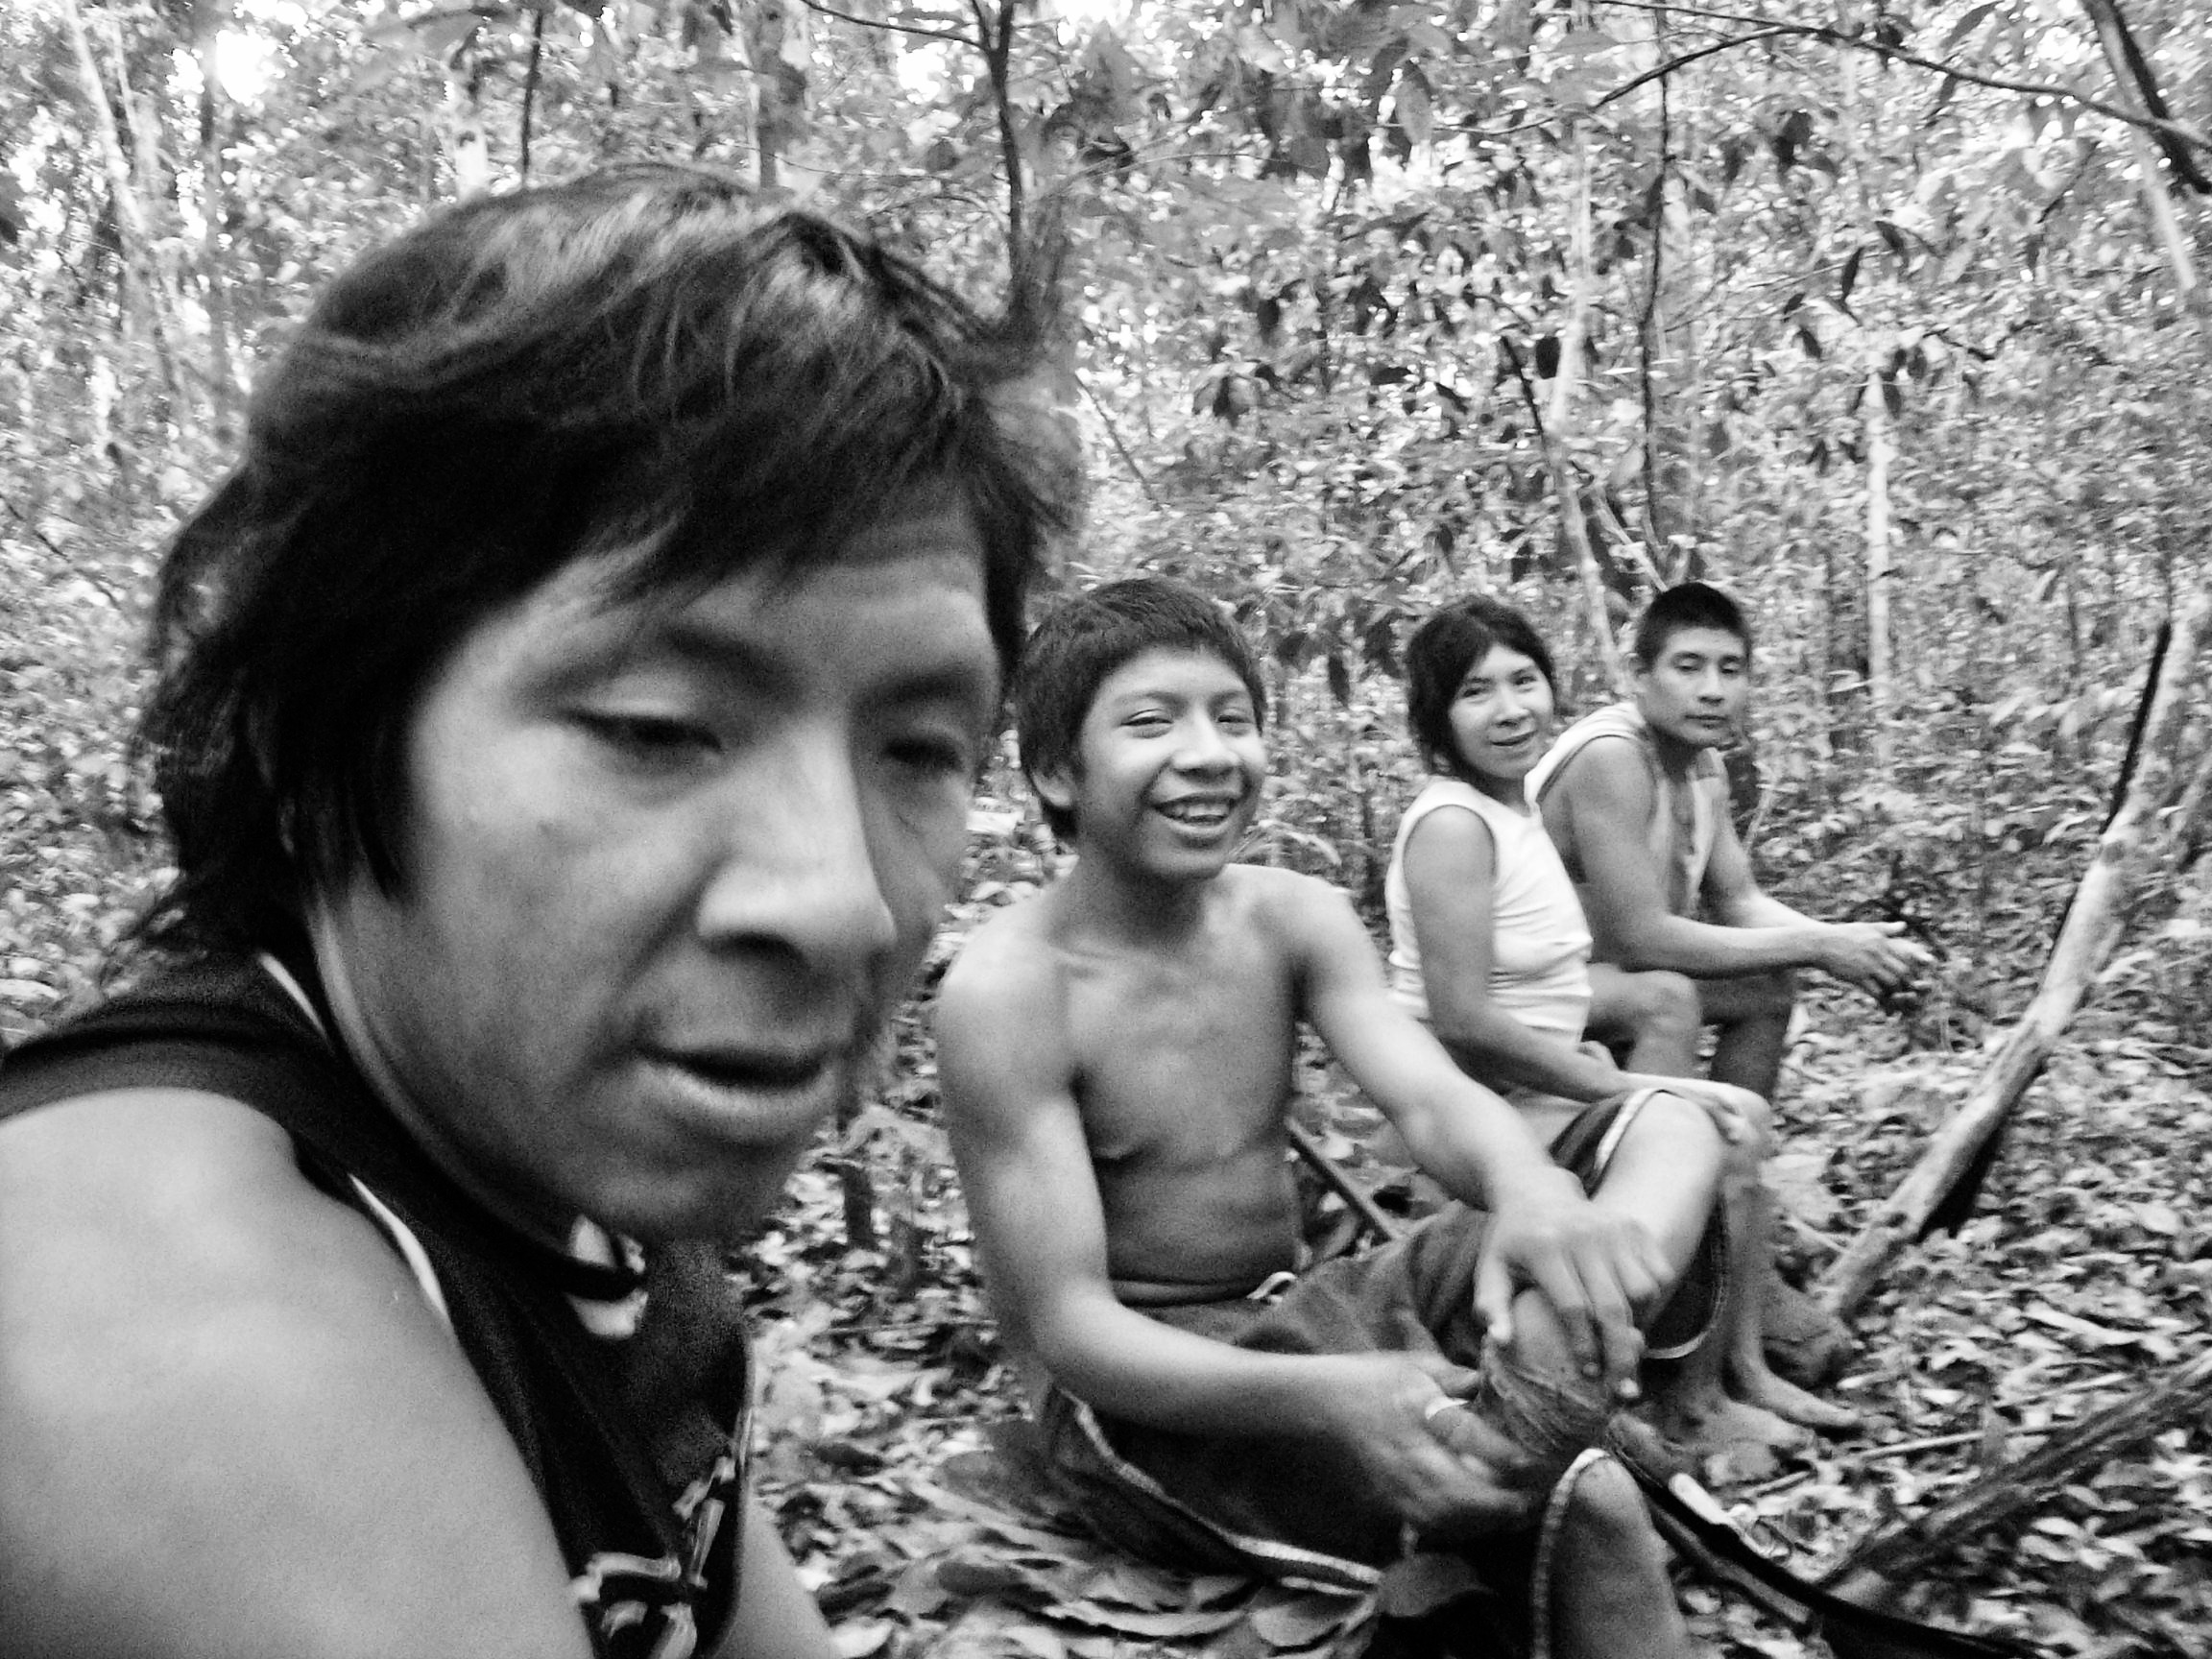
\includegraphics[width=\textwidth]{./imgs/100_5648}
\caption{Na floresta, descansando durante uma caçada, Uriximatỹa (primeiro plano), Jui’i
sorrindo ao lado de sua mãe Ajrua e seu pai Uirahoa (aldeia Juriti, 2007).}
\end{figure}

\section{Distâncias}\label{distuxe2ncias}

As distâncias sociais (e genealógicas) entre os seres humanos
(\emph{awatea}) são pensadas mediante as ideias \emph{harapihiara} e
\emph{harapihianã}. \emph{Harapihiara} (\emph{ha}-\emph{r"-apihiar"-a}) é
um termo formado pelo pronome clítico de 1ª pessoa \emph{ha}; o termo
\emph{apihia(r)}, que pode ser traduzido por ``aquele que está próximo''
(como veremos melhor no próximo capítulo); e o sufixo nominal
-\emph{a}\footnote{Trata"-se do sufixo nominal -\emph{a}, que ocorre com
  raízes nominais tornando"-as capazes de exprimir nomes com referência.
  Sem esse sufixo, os nomes funcionam como predicado (p. ex. \emph{hamymy} ``eu tenho filho(a)'', enquanto \emph{hamymyra} ``o meu
  filho(a)'') ou como vocativo (\emph{hamymy, aju kurupi!} ``meu filho,
  venha cá!'') (Magalhães, comunicação pessoal). O sufixo nominal
  -\emph{a} é muito produtivo na língua Guajá em palavras como
  \emph{tatu"-a} (o tatu), \emph{kwaxi"-}a (o quati) e \emph{kwarahy"-a} (o
  sol) e pode ocasionar a recuperação de uma consoante final oculta na
  raiz do nome, -\emph{r ou -}n, como em \emph{karawar"-a} (o
  \emph{karawara}), \emph{harapihiar"-a}, como vimos acima, ou
  \emph{amỹn"-a} (a chuva).}. Já no termo \emph{harapihianã}
(\emph{ha"-r"-apihia"-nã}), o sufixo -\emph{nã} denota inautenticidade
(``falso''), fazendo com que \emph{harapihianã} seja algo traduzido como
um ``falso próximo''. E por meio desta pequena diferença os Guajá
distinguem ``consanguíneos e afins `próximos/reais' daqueles
`distante"-classificatórios''' (Viveiros de Castro, 2002a, p. 130). Esses
termos ganham, de forma geral, uma ampla acepção. \emph{Harapihiara}
pode ser, por exemplo, os tubérculos que crescem juntos em uma mesma
raiz. Ou as frutas de uma mesma árvore são concebidas como \emph{irmãs}.
E por \emph{harapihianã} podem ser tratados animais com morfologia
parecida, segundo os Guajá, como ainda veremos no capítulo 6. Trata"-se
portanto de termos de relação para os mundos humanos, animais e
vegetais, e não categorias estritas ao ``sistema de parentesco''. Para
os humanos (\emph{awa}), as pessoas de sua aldeia e as ligadas a
parentes destas podem ser \emph{harapihiara} (``próximos'') ou
\emph{harapihianã} (``distantes''); da mesma forma, seres não humanos que
incorporam a suas relações (sejam animais de criação ou os
\emph{karawara} celestes) também são tidos como \emph{harapihiara} ou
\emph{harapihianã}, a depender da proximidade. E diferentes seres no
mundo, para além dos humanos, mantêm entre si relações do tipo
\emph{harapihiara} ou \emph{harapihianã}.

Como ideias de relação (e não recursos vocativos), os termos
\emph{harapihiara} e \emph{harapihianã} organizam o universo dos
parentes, dividindo"-o em duas categorias básicas, ``os próximos'' e os
``distantes'', que, em conjunto, formam a humanidade como um todo,
\emph{awatea} (``gente de verdade''). Desta forma, a definição baseada na
macro oposição ``afins/consanguíneos'' não colabora para o entendimento
destas duas categorias, pois o sistema de aliança Guajá, como veremos,
embora também gravite em torno dessas duas ideias, permite que ambas
possam indicar ora ``afinidade'', ora ``consanguinidade'', uma vez que ``a
distinção entre o próximo e o distante é característica de socialidades
em que a residência predomina sobre a descendência, a contiguidade
espacial, sobre a continuidade temporal'', como é o caso em questão (ver
Viveiros de Castro, 2002, p. 130).

Doravante, ao discutir as ideias de \emph{harapihiara} e
\emph{harapihianã}, farei referências a distinções variadas (e
complementares), tais como as que vimos acima, devido ao caráter
polissêmico dessas duas categorias, que ora remetem a um código
espacial, ora temporal, e ora diametral/concêntrico. No entanto, a ideia
que conduz minha análise se baseia, fundamentalmente, nas ideias de
``proximidade'' e ``distância'' --- genealógica, espacial e cognática --- tal
como define Viveiros de Castro (1993 e 2002). No caso específico Guajá,
o que distingue essas duas categorias é o sufixo -\emph{nã,} que denota
inautenticidade e pode ser encontrado na formação de outros termos
referentes de parentesco, como:

\begin{center}
\versal{F} = \emph{tu} \emph{→} \versal{FB} = \emph{tu-nã}\medskip

\versal{M} = \emph{ihí →} \versal{MZ} = \emph{ihi-nã}
\end{center}

Assim, ambos os sexos reconhecem o pai (\versal{F}) como \emph{tu} e o irmão do
pai (\versal{FB}) como \emph{tu"-nã}; e uma vez, ao lhes perguntar sobre tal
classificação, me disseram que a tradução de \emph{tuna} seria ``pai
pouco'' ou ``pai fraco''. O mesmo ocorre para a irmã classificatória de um
homem. Enquanto irmã é referida por \emph{hajnawãi}, uma mulher que seja
tida como irmã de um homem (por ele ter casado com sua filha, por
exemplo) é chamada \emph{hajnawajnã}. Tais soluções podem ser vistas em
outros casos amazônicos, como entre os Waimiri"-Atroari, em que parentes
colaterais (\versal{FB} e \versal{MZ}) ganham o tecnônimo -\emph{kî} marcando essa
diferença, assim \versal{F} = \emph{yimî} e \versal{FB} = \emph{yimkî}. Trata"-se aqui ``do
reconhecimento, no plano terminológico, de dois \emph{graus de distância
lateral} entre parentes consaguíneos, a oposição
linearidade/colateralidade é colocada como um epifenômeno da oposição
'proximidade/distância''' (Silva, \emph{op. cit.}, p. 47). Tudo se passa como se
houvesse uma projeção do sistema perto/longe que rege essas relações em
todos os níveis de relação chegando até mesmo à consanguinidade. A
partir dessa ideia e enfatizando o gradiente de proximidade/distância
que sobredetermina os termos \emph{harapihiara} e \emph{harapihianã}
(como veremos neste e nos próximos capítulos), podemos traduzi"-los tanto
por ``próximos/distantes''; ``lineares/colaterais''; ``cognatos/aliados'';
``consanguíneos/afins''; ``corresidentes/não corresidentes''; e, como parece
confirmar a língua Guajá, ``verdadeiros/falsos (classificatórios)''. Por
isso minhas definições oscilarão a partir destas múltiplas ideias que
compõem essa complexa oposição (\emph{harapihiara}/\emph{harapihianã}),
e os exemplos e casos que trarei neste e nos próximos capítulos
determinarão o código a que me estarei referindo. Além disso, podemos
pensar os termos \emph{harapihiara} e \emph{harapihianã} como
macrocategorias, uma vez que eles fazem referência a conjuntos muito
diferentes de relações que vão desde as de parentesco, propriamente, até
a relação entre um animal de criação e seu dono; duplos celestes e
terrestres; partes de um vegetal; um nome e o ser nominado, dentre
outras situações que envolvem seres humanos e não"-humanos de diferentes
ordens.

Não pretendo discutir aqui o sistema de parentesco (tema do próximo
capítulo), mas, sim, uma terminologia de relações que extrapola o campo
do parentesco e constitui um idioma que informa diferenças e
semelhanças; identidades e diferenças; \emph{harapihiara} e
\emph{harapihianã}.

\section{Proximidades}

\emph{Harapihiara} é o termo mais próximo à ideia de um ``nós
cognático''\footnote{Para essa ideia, ver Albert (1992).}, do tipo
``parentes verdadeiros'', cujo casamento é proibido, enquanto
\emph{harapihianã}, além de abranger a classe das pessoas próximas,
porém passíveis de se casar (esposas, maridos, cunhados, sogras, genros
e assim por diante), abrange outras pessoas (\emph{awa}) ``amigas''
(\emph{hary} ou \emph{aty}) e ``desconhecidos'' que, uma vez incorporados
via casamento e/ou corresidência a um grupo local, podem ser
potencialmente \emph{harapihianã}, tal como encontramos em diversos
casos amazônicos. Para um homem, os \emph{harapihiara} mais próximos de
sua geração são seu irmão (\versal{B}) e seu primo paralelo paterno (\versal{FBS}). Para
uma mulher, seria sua irmã (\versal{Z}) e suas primas paralelas bilaterais (\versal{MZD}/
\versal{FBD}). Por isso, o termo utilizado por ego masculino para \versal{B}/\versal{FBS} e por ego
feminino para \versal{Z}/\versal{MZD}/\versal{FBD} é \emph{harapihiara}, obedecendo"-se a
equivalência dos sexos.

A totalidade dos termos de parentesco Guajá (como veremos no próximo
capítulo), tanto para ``afinidade'' quanto para ``consanguinidade'', se
encaixa em alguma destas duas ideias (\emph{harapihiara} e
\emph{harapihianã}), assim como qualquer relação entre seres humanos
(\emph{awa}) é regida por um ou outro desses termos. Como sabemos, o
componente genealógico e/ou socioespacial é parte constituinte do
dravidianato amazônico, atuando como vetor nessas relações e fundamental
à compreensão desses sistemas (ver Viveiros de Castro, 2002, p. 121;
Silva, 1995; Taylor, 1996; Gow, 1991). Desta forma, para o caso em
questão, os termos \emph{harapihiara} e \emph{harapihianã}, funcionam
para exprimir as ideias de parentes ``próximos'' ou ``verdadeiros''
(\emph{harapihiara}) e ``distantes'' ou ``classificatórios''
(\emph{harapihianã}). E, apesar do fato de se referirem a diferentes
relações, o conteúdo dessas não está relacionado à sorte automática (e
binária) refletida na oposição ``afins''/ ``consanguíneos''. Assim, no caso
Guajá, alguns indivíduos que são \emph{harapihiara} entre si podem sê"-lo
por laços de aliança ou amizade, ocorrendo, inclusive, em relações entre
indivíduos do sexo oposto, como veremos no caso abaixo.

Em todos os anos de fuga que viveram os Guajá, quando evitavam o contato
e adotavam estratégias de viver entre si, essas ideias estavam operando;
ao serem transferidos para uma aldeia após os contatos, diversas pessoas
que não se conheciam anteriormente passaram a se reconhecer como
parentes próximos ou distantes, e assim as vidas nas aldeias foram
recomeçadas. Panaxĩa e Pira'ima'ã viviam em grupos locais distantes
entre si até a época do contato entre a \versal{FUNAI} e o grupo de Panaxĩa, em
1996, quando se juntaram às outras famílias que já viviam na aldeia
Juriti. Pira'ima'ã se casou com a filha de Panaxĩa, Pakwa'ĩa, e desde
então os dois passaram a se classificar como germanos de sexo oposto.

\begin{figure}[H]
\centering
  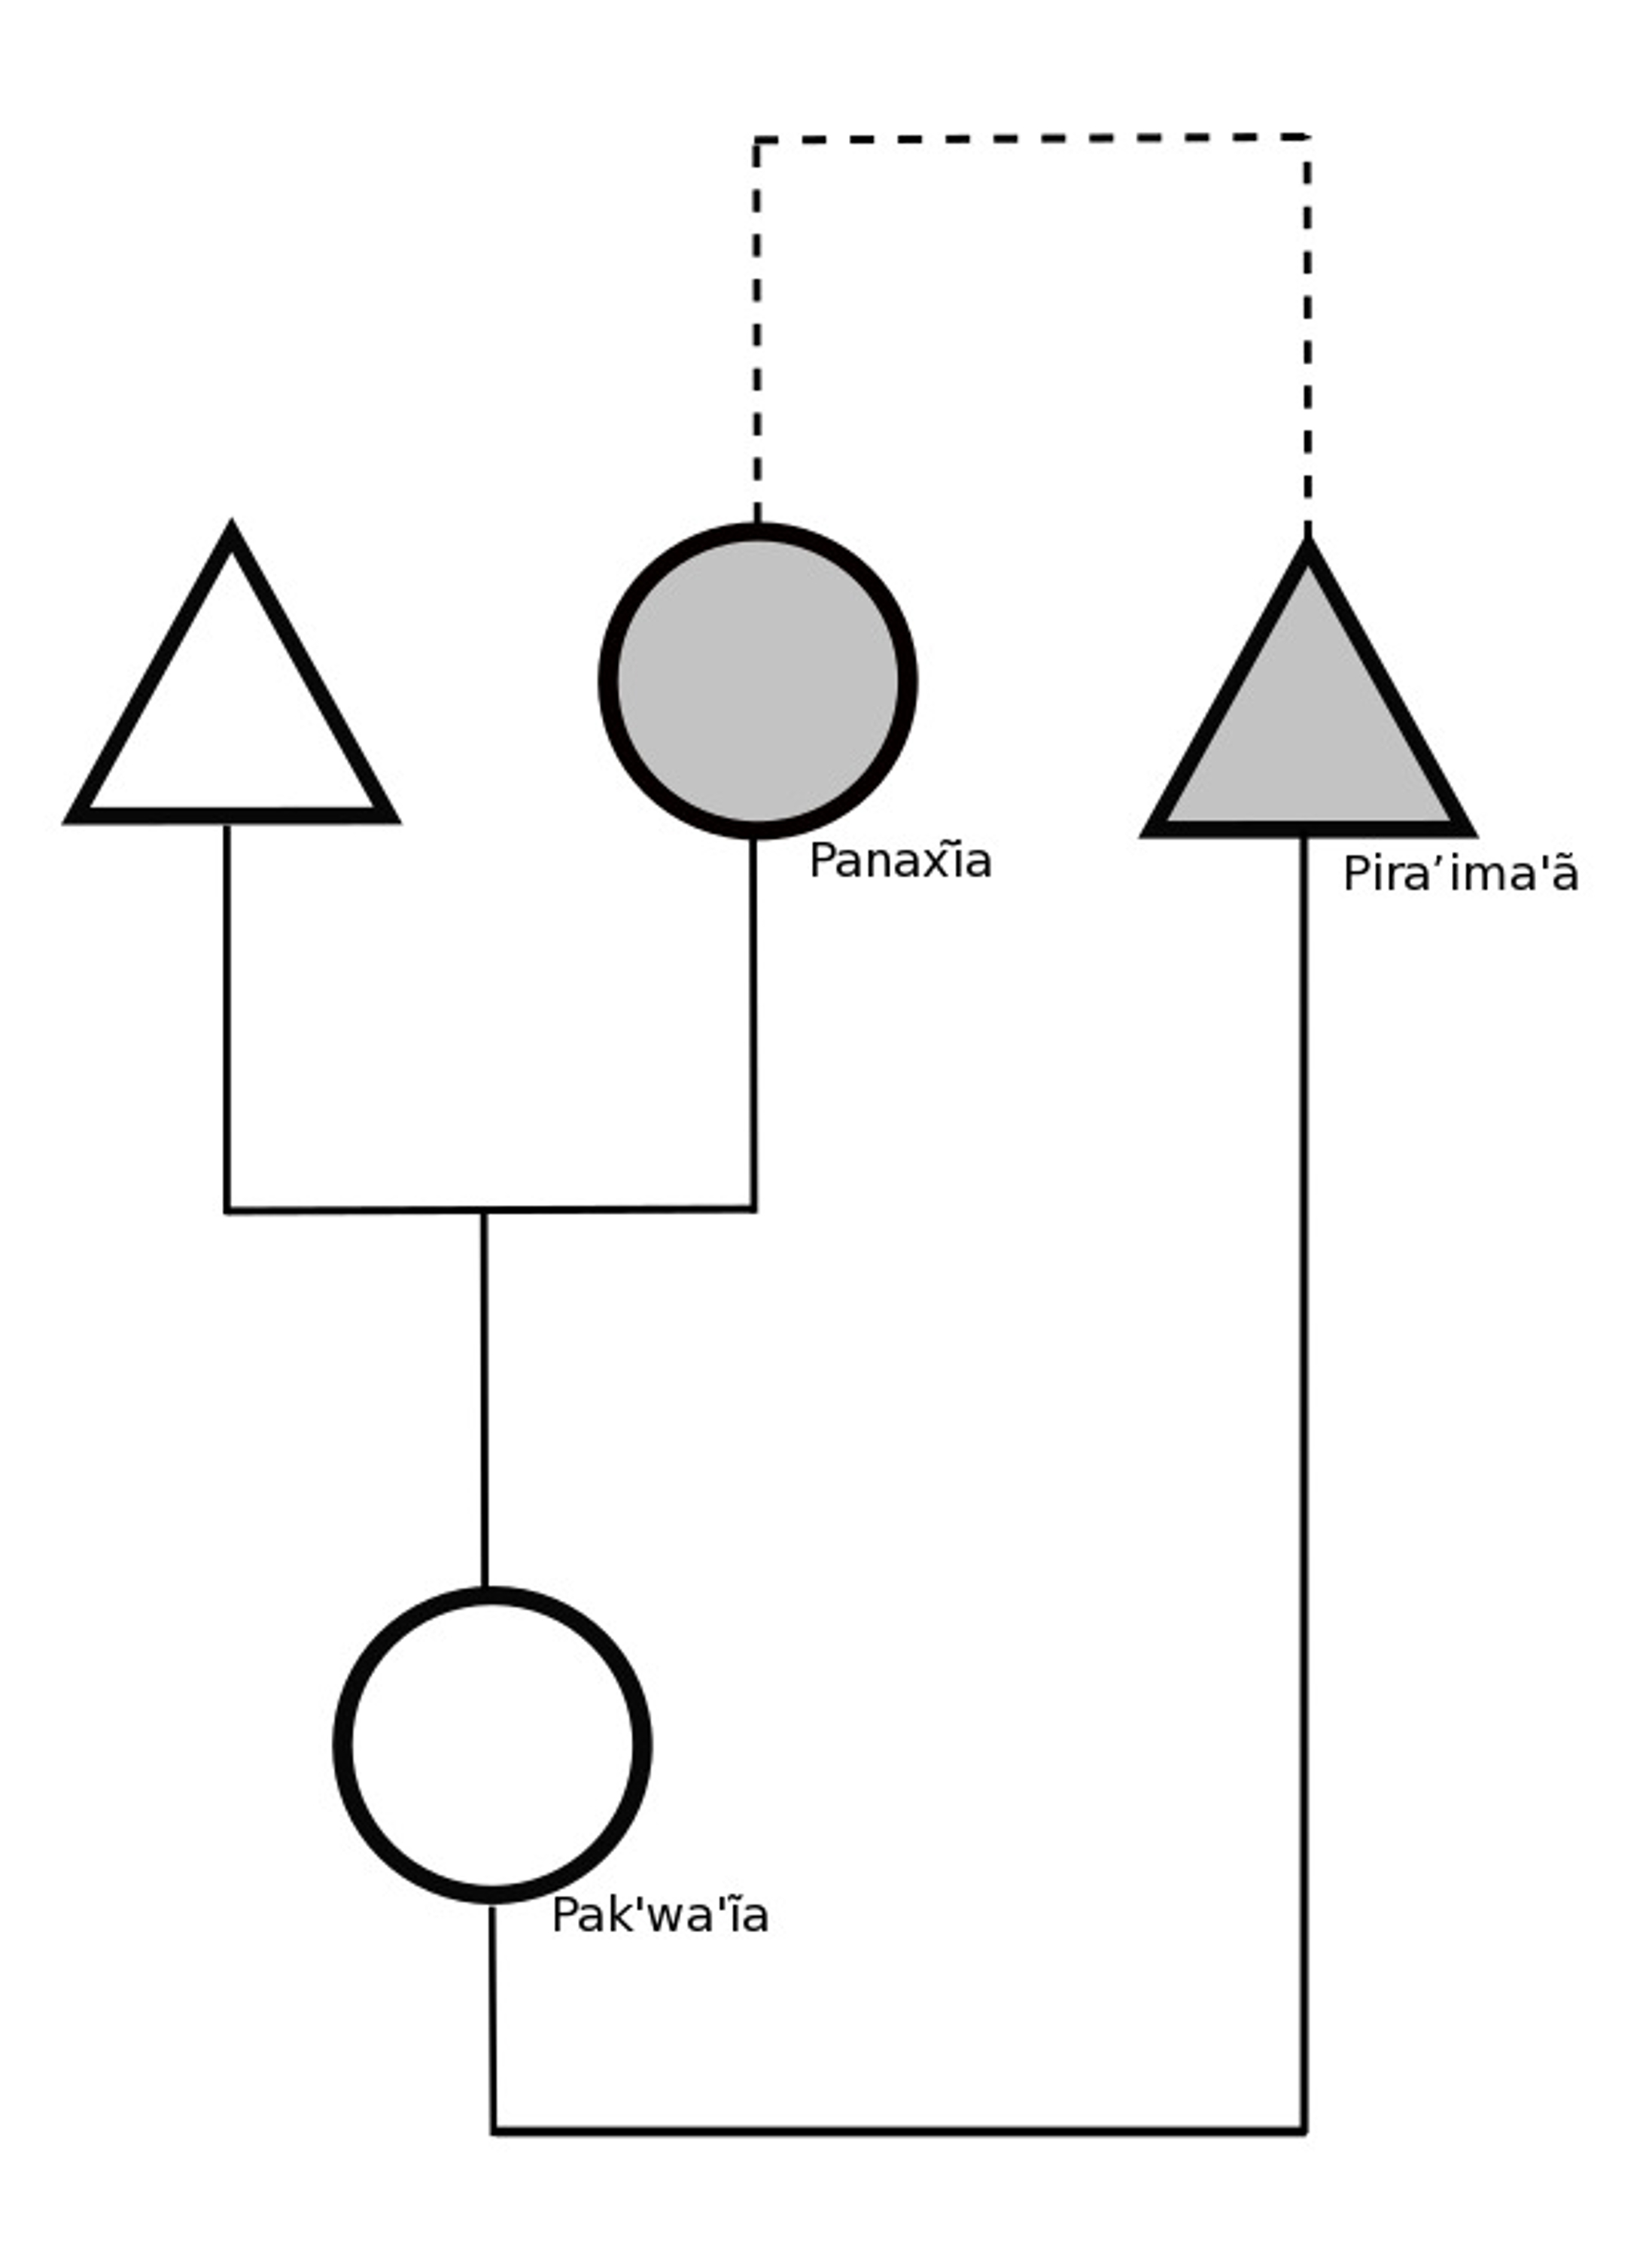
\includegraphics[width=75mm]{./imgs/Figura_5_crop}
%\caption{Figura 5}
\end{figure}

Discutirei essa característica do sistema de aliança Guajá no próximo
capítulo, porém gostaria de, por ora, frisar que dois indivíduos, até
então separados pela genealogia e pela distância física, passaram a
estabelecer entre si uma relação de proximidade, condensada na ideia de
\emph{harapihiara}, quando, antes de uma sucessão de eventos, eram
considerados ``distantes'' (\emph{harapihianã}). Tal mudança na forma de
relação é recorrente entre os Guajá e, longe de representar uma
indeterminação dos termos que se alternam em circunstâncias diferentes,
demonstra que as diferenças entre pessoas ``casáveis'' e
``não"-casáveis'' ou ``parentes próximos'' e ``distantes'' não estão
presas a categorizações fixas --- ``o que impede que se pense a pragmática
social em termos de uma subordinação simples à sintaxe terminológica''
(Viveiros de Castro, \emph{op. cit.}). Se o gradiente de distância é
fundamental para as classificações do parentesco na Amazônia, para um
povo como os Guajá (dentre tantos outros) esta pode ser encurtada ou
estendida ao sabor do tempo e/ou da memória, modificando as relações
atuais. Em poucas palavras, um \emph{harapihianã} pode se tornar um
\emph{harapihiara}, e --- com menos frequência --- vice"-versa. Todas as
relações entre humanos (\emph{awa}) e toda a humanidade --- ela mesma ---
estão pautados por essa oposição.

\section{Das formas de existência}\label{das-formas-de-existuxeancia}

Vivendo isolados, distantes uns dos outros, desde antes do contato até
os dias atuais, os diferentes grupos locais não formam um ``conjunto
homogêneo Guajá'', tal como prescreve uma idealização de ``grupo
indígena'', com intercâmbios intercomunitários, autoidentificação com o
``grupo'' e alianças em diferentes situações. A forma pela qual os Guajá
sempre se organizaram, sem grandes aldeias ou assentamentos, é reflexo
de socialidade particular, que privilegia formas independentes e
``fragmentárias'' de organização social, marcadas inclusive pelo
estranhamento entre esses pequenos coletivos. Mesmo nos dias atuais, em
que diferentes famílias foram reunidas em uma mesma aldeia, as próprias
aldeias são separadas em setores baseados em grupos de homens
importantes (\emph{tamỹ}, ``chefes'') e, após décadas, repartidos em
quatro aldeias, as pessoas estão se dividindo continuamente em novas
aldeias --- três novas apareceram nos últimos anos (sete no total), e não
sabemos quantas ainda virão.

Por exemplo, Ajrua e Juriximatỹa, na década de 1980, antes do contato,
viviam junto com o grupo de Amỹ Pirawãja, mãe de diversos homens
importantes da \versal{TI} Caru, mas os anos de fuga os separaram e, postos em
aldeias distantes uma das outras, estão há mais de duas décadas sem se
ver, embora, genealogicamente, se acreditem \emph{harapihianã},
``parentes próximos''. Próximos no passado, distantes no presente, o grupo
da aldeia Juriti se refere às pessoas das outras aldeias como de ``boca
diferente'' (\emph{amõa} \emph{irua}), ou de um ``falar ruim'' (\emph{i' ĩ}
\emph{manyhỹ}), devido às mínimas variações dialetais encontradas em
cada uma dessas aldeias. Antes do contato, partindo"-se de qualquer
\emph{haripa} (``minha casa"-aldeia"-acampamento''), os \emph{harakwaha}
mais distantes eram totalmente desconhecidos, assim como os grupos que
neles habitavam. Embora guardem uma história social comum, com dramas e
episódios bastante parecidos, as pessoas de cada região experimentaram
vidas e fugas diferentes, uma vez que sempre viveram afastados uns dos
outros.

No passado, os grupos sem contato evitaram ao máximo o encontro com os
\emph{karaia} (não indígenas), e mesmo havendo outros Guajá contatados
incorporados às frentes de atração, nem sempre isso resultava no sucesso
dessas frentes. Os que estavam na mata desconfiavam da condição de
humanos verdadeiros (\emph{awatea}) dos contatados, já que um dos medos
dos ``isolados'' (chamados \emph{mihua}) , além das doenças, era perderem
suas mulheres para esses \emph{awa} ``amigos dos \emph{karaia}''
(\emph{karai rapihianã}), que podiam tanto ser ``parentes''
(\emph{awatea}) quanto inimigos (\emph{mihuatea} ``desconhecidos''). O
temor dos ``isolados'' de perder suas esposas está longe de ser infundado,
tendo"-se em vista que um dos principais interesses dos homens Guajá que
participam das frentes de atração, até hoje, é a possibilidade de
conseguir novas esposas. Quando da criação do \versal{PIN} Juriti, em 1989, além
do intérprete To'oa que ajudou no contato, outros homens da aldeia
``Awá'', como Kamajrua, foram lá viver. To'oa casou"-se com Amỹ Pirahỹ, que
fazia parte do pessoal recém"-contatado, fixou residência na nova aldeia
e passou a exercer certa liderança entre o grupo recém"-contatado ---
principalmente nos assuntos referentes à relação com a \versal{FUNAI}, o trabalho
na roça, etc. Além disso, outro homem, Takamỹ, que vive na aldeia
\emph{Awá}, tomou como esposa uma outra jovem desse grupo e voltou a
viver em sua aldeia original, sem nunca mais voltar à Juriti\footnote{Dada
  a complexidade envolvida em um esquema de viagem intercomunitária, os
  Guajá da aldeia Juriti quase nunca saem para visitar outras aldeias,
  mesmo que tenham parentes vivendo nelas. Uma vez que não existem
  acessos às outras aldeias por dentro do território, qualquer viagem
  entre a aldeia Juriti e as do Pindaré implica sair da jurisdição das
  Terras Indígenas por transportes oficiais (\versal{FUNAI} ou Funasa), dormir em
  cidades (na casa de algum funcionário ou hotel), ter gastos com
  alimentação e (muitas vezes) roupas, dentre outras providências que os
  Guajá, sozinhos, não têm meios de viabilizar.}.

Ontem e hoje as diferenças continuam marcadas pelos tipos de relação que
cada um dos grupos das diferentes aldeias estabelece. Como já mencionei,
a maior parte de minha pesquisa de campo foi desenvolvida na aldeia do
\versal{PIN} Juriti, uma comunidade pequena que em 2013 contava com 66 pessoas.
Como escrevi anteriormente, quase tudo o que aprendi com os Guajá se deu
entre essas pessoas, inclusive suas ideias sobre os outros grupos
humanos que viviam em outras comunidades e que com eles tinham
pouquíssimo contato, a não ser quando iam (quase sempre por motivos
médicos) para Santa Inês (ou mesmo para São Luís). Em diversas situações
me lembravam como eles são diferentes dos Guajá das outras aldeias
(``Tiracambu'', ``Awá'') e, sem mencionar os moradores da aldeia do \versal{PIN}
Guajá (aldeia do Cocal), caso extremo de estranhamento para os Guajá do
Juriti, me diziam estarem ``doidos'' (\emph{wakyhy}) por beber cachaça e
fumar cigarro, tal como fazem os Tenetehara e os Ka'apor\footnote{Por
  não usarem tabaco, os Guajá falavam mal dos Tenetehara e os Ka'apor
  por fazê"-lo. Além disso, diziam"-me que não fumavam porque lhes faria
  muito mal.}.

As pessoas da aldeia Juriti maldiziam as das aldeias Awá e Tiracambu por
terem feito alianças com os Guajajara (Tenetehara), uma vez que sempre
mantiveram com os Tenetehara uma relação de desconfiança, devido a
conflitos passados. Em diversas ocasiões sugeriram que eu ``desistisse''
de realizar meu trabalho de campo junto aos Guajá do Pindaré (aldeias
Awá e Tiracambu), uma vez que os de lá, por estarem ``misturados''
(\emph{iku} \emph{pamẽ}) com os Guajajara, também estariam bebendo e
fumando muito. No entanto, quando cheguei à aldeia Tiracambu, as pessoas
de lá me pediam justamente para que eu não retornasse à aldeia Juriti,
pois, devido a seu relativo isolamento, era um lugar desconfortável e
difícil de chegar. Falavam também que meus amigos da aldeia Juriti
seriam ``gente do mato'' (\emph{awa} \emph{ka'apahara}), ou mesmo
\emph{awatea}, ``gente de verdade'', que nesse sentido era sinônimo de um
tipo de existência (onde se vivia nu, dormindo em tapiris, sem
agricultura e fugindo) que as outras aldeias não querem mais
experimentar.

O resultado dessa diferenciação é que tais ``parentes'', entre si, seriam
\emph{amõ awa} (``outros Guajá''). Devido às diferenças
político"-geográficas desde a aldeia Juriti, todo tipo de críticas aos
Guajá do Pindaré (aldeias Awá e Tiracambu) me foram relatadas --- a fim de
me dissuadir de uma possível aproximação com as outras aldeias ---, e a
principal delas é que as pessoas alardeariam minha presença para os
Guajajara, com o intuito de eles me expulsarem da terra indígena. Para
evitar isso, pediram para que eu não passasse longas temporadas naquelas
aldeias; e, ainda, para que eu tivesse cuidado com minha alimentação,
pois os Awá das outras aldeias comiam animais que eles haviam descartado
de sua dieta, como preguiças, onças e sucuris --- alegando que os Guajá do
Pindaré são dotados de um fígado (\emph{ipia'akera}) diferente do deles,
mais preparado para tolerar tais carnes; dentre outras observações.

Forline (com. pessoal) conta que, no ano de 1993, a administração da
\versal{FUNAI} resolveu abrir uma trilha por dentro da \versal{TI} Caru que ligasse a
aldeia do \versal{PIN} Awá à do \versal{PIN} Juriti\footnote{Nesta época, os Guajá estavam
  sob a administração regional da \versal{FUNAI} de Belém, que tomava decisões
  (ainda mais) autoritárias e sem qualquer critério razoável no que
  dizia respeito ao processo de contato e estabelecimento em aldeias dos
  grupos Guajá isolados.}, como que para propiciar uma espécie de
``intercâmbio'' entre aldeias tão distantes (incluindo"-se matrimônios e
alianças para maior vigilância da área indígena). A viagem, que durou 13
dias por dentro da floresta, partiu da aldeia Juriti em direção à aldeia
do \versal{PIN} Awá, atravessando uma região repleta de morros. Na equipe, além
dos funcionários da \versal{FUNAI}, estavam muitos jovens da aldeia Juriti, além
da família de Takwarẽxa'a, contatada no ano anterior. Porém tal
iniciativa só gerou mal"-estar entre as aldeias: algumas pessoas estavam
com gripe (e tuberculose) e acabaram trocando (não mulheres, mas)
doenças. A, então, jovem Pikawãja, irmã de Wirahoa, foi pega
(\emph{pyhy}, ``tomar'') em casamento por Takamỹ, da aldeia do \versal{PIN} Awá.
Algumas pessoas do \versal{PIN} Awá ameaçaram de morte os Guajá do \versal{PIN} Juriti,
pois não gostaram que muitos deles se enamoraram por mulheres de lá,
dentre outros entreveros. Nesse ínterim, o coordenador da expedição,
Fiorello Parisi, percebeu que sua ideia não havia sido bem"-sucedida e
foi embora, deixando para trás um quadro de animosidade para eles
resolverem entre si. O resultado foi que as pessoas da aldeia Juriti
usaram o mesmo caminho de ida para voltar a sua aldeia; perderam uma
mulher e ainda foram ameaçados de morte.

Durante os meus períodos de campo na aldeia Juriti, eu tinha por missão
informá"-los sobre como estão (ou melhor, são) as pessoas da aldeia
Tiracambu; e o inverso também ocorria. O principal interesse do grupo da
aldeia Tiracambu era minha experiência entre os Guajá da aldeia Juriti.
Ambos me questionavam: se os outros tinham bastante caça; como eram suas
roças; como eram as estruturas da \versal{FUNAI}, ; se havia mulheres; como eram
as crianças; se eram nervosos (\emph{imahy}) ou calmos (\emph{katy},
``bons''); dentre outras inúmeras indagações. As diferenças entre esses
grupos Guajá variam em atitudes, dieta, e chegam a pequenas diferenças
na fala que, muitas vezes, os Guajá da aldeia Juriti diziam ser
imensuráveis. Vejamos algumas.

\section{Comida}\label{comida}

\emph{Awa nimi'ũa}, ``comida de gente'' (entendida por carnes variadas,
mel, frutos e também farinha, arroz, bolachas, dentre outros), se opõe,
por exemplo, a \emph{karai nimi'ũa}, ``comida dos não"-indígenas'', repleta
de sal e carnes que os Guajá ``não sabem'' comer da maneira apropriada,
como a carne de gado e frango, pois poderia fazer mal. Ou \emph{awa mihu
nimi'ũa}, ``comida de índio brabo'', se refere à sub"-dieta pela qual
passam os Guajá que vivem em isolamento voluntário, cheia de animais
nocivos (como cobras e ratos), tubérculos (como cará"-do"-mato) e frutos
(como a pequirana) que as pessoas da aldeia não toleram hoje em dia ---
esta é uma dieta de ``antigamente'' (\emph{imỹna}).

Ao mencionar as diferenças internas à uma comunidade Guajá, Cormier
lembra que o fato de diferentes grupos terem sido trazidos para viver
juntos na reserva Caru fez com que cada um deles trouxesse um padrão
diferente de alimentação, e, embora próximos uns dos outros, eles
diferiam em pequenas coisas. Dessa forma, alguns tinham mais receio de
comer determinados alimentos do que outros (Cormier, \emph{op. cit.}, p. 40).
As diferenças alimentares marcam as distâncias que separaram os grupos
Guajá durante toda a sua história, do passado ao presente. Dos animais
de que os Guajá se alimentam (ver Forline, 1997; ver também Cormier,
2003), à exceção dos que os humanos nunca comem (como, por exemplo,
corujas, urubus, morcegos, gambás, raposas, coelhos e
esquilos/quatipuru), os \emph{awa} são muito tolerantes a sabores,
texturas e eventuais toxidades que um alimento possa carregar; e por
mais absurdo que possa parecer é muito difícil fechar uma relação de
animais interditos. Até 2013 eu não sabia do consumo de capivara
(\emph{kapijawara}), mas Warixa'á, que vive na aldeia Awá, disse que ele
e alguns homens comiam, mas realmente é uma carne ``reimosa''
(\emph{manahỹkera}), proibida às mulheres, e nem todos os homens a
toleram. Sobre as onças, podia se dizer o mesmo: na aldeia Awá, até as
onças pintadas podiam ser matéria de consumo de alguns coletivos, ao
passo que na aldeia Juriti, mesmo a suçuarana (que todos dizem ter uma
carne saborosa como a do veado) era consumida por poucas pessoas e ainda
com parcimônia. No limite, a dieta reflete algo fundamental de toda a
socialidade \emph{awa} que impossibilitaria fecharmos uma ideia geral de
``sociedade'' ou ``povo'' como um todo homogêneo. Afinal, sabemos ---
desde autores como Marilyn Strathern, em \emph{O gênero da dádiva}, por
exemplo --- que a \emph{Sociedade} seria mais um problema de ``nós'',
antropólogos, do que de nossos interlocutores (Strathern, 1988, p. 3).

Muitos animais são apreciados por alguns e desprezados por outros, a
depender da aldeia. Após o contato, com a junção de diferentes grupos
locais em um mesmo lugar, a tendência seria que em cada aldeia a dieta
se estabilizasse e que animais antes apreciados fossem descartados por
motivos variados --- que vão desde a pouca quantidade de gordura até a
nocividade de determinada substância ao corpo humano, passando pelo
sabor e consistência. O fato de alguns Guajá comerem o que os de outra
aldeia não comem não passa por uma noção do tipo ``tabu'', mas, como eles
mesmos propõem, uma diferença congênita (tal como sabemos há algum tempo
a respeito da corporalidade dos povos amazônicos --- ver Seeger \emph{at
all}, 1979) que, nesse caso, é expressa pela ideia dos diferentes tipos
de fígado (\emph{ipia'akera}) das pessoas. Quando algumas pessoas da
aldeia Juriti afirmam nunca terem consumido determinados alimentos, não
é possível generalizar o argumento para todos os outros Guajá, nem mesmo
daquela mesma aldeia. Certa feita, ao matarem um tamanduá
(\emph{tamanawã}), animal cujo sabor era de duvidoso apelo culinário --- e
sempre disseram não gostar, pois afirmam fazer mal (\emph{manahỹ}), além
de ser fedorento (\emph{irymyhỹ}) e reimoso (\emph{manahỹkera}) ---, dois
homens mais velhos, além de consumir o tamanduá ofereceram"-no a alguns
rapazes para experimentarem. Outros homens adultos me disseram que não
comeriam, pois, desde sua mudança para o posto indígena, não mais se
interessavam por carnes como aquelas consideradas \emph{manahỹ}
(``ruins'', ``feias'') e \emph{iramyhỹ} (``fedorentas''). O mesmo ocorreu com
uma suçuarana (\emph{jawaraporõ}) --- animal que consumiam antes do
contato --- que, depois de abatida, alguns cogitaram transportar para a
aldeia para comê"-la, porém foram dissuadidos por outros por acharem que
não valeria a pena, uma vez que estávamos no meio de uma viagem para um
acampamento de caça. Carnes como a de tamanduá"-bandeira
(\emph{tamanawã}), suçuarana (\emph{jawaraporõ}), porco"-espinho
\emph{kwanũa} (cuandú/ouriço"-cacheiro --- \emph{Coendou prehensilis}) e
tamanduá"-de"-colete ou a mambira (\emph{tamãnawã'ía} --- \emph{Tamandua
tetradactyla}) têm suas qualidades de bom alimento (além da segurança da
ingestão) postas à prova e figuram no grupo das pouco apreciadas, por
``fazerem mal''; mas podem ser consumidas por alguns, principalmente
entre os que assim faziam antes do contato.

O quati (\emph{kwaxia}), da mesma forma, tem uma carne bastante
apreciada, principalmente devido a seu potencial gorduroso. Nos meses de
inverno, época da oferta de gordura nos animais (\emph{ikira ra'o} ---
``muito gordo''), o quati é consumido por todos, porém alguns cuidados no
manuseio dessa carne devem ser observados. Diferentemente de outros
animais (como macacos), dos quais se aproveitam as vísceras
(\emph{ha'aikera}) como aperitivo (principalmente entre os velhos), o
quati deve ser manuseado e limpo (\emph{hape}) em separado das outras
carnes, dado o ``fedor'' (\emph{irymyhỹ}) que exala. Embora para meus
limitados sentidos o cheiro das vísceras do quati não diferisse do de
outros animais do mesmo porte (como os tatus), meus amigos distinguiam
muito bem seu odor, que tem faculdades/cheiros patogênicos
(\emph{mixahy}) e afeta diretamente a saúde humana. Devido aos possíveis
danos à saúde, quem o limpar deverá cuspir a todo momento para que o
cheiro não penetre na própria carne nem adoeça. Quase sempre o limpam
longe da cozinha, de preferência em uma área do rio destinada a isso,
lavando"-o para que fique purificado, sem o odor das vísceras. Só assim
sua carne estará pronta para consumo. Certa ocasião, quando eu estava
com um grupo de pessoas na casa de Wirahoa, Juxa'a voltava do rio em
direção ao moquém com dois quatis já bem limpos. Ao passar por nós,
todos começaram a cuspir com receio de que o odor do animal ainda lhes
viesse a fazer mal. Uma das explicações, como já observei, é o fato de
os quatis, assim como os gambás, estarem relacionados aos espectros
\emph{ajỹ.}

Outros animais que também figuram no grupo de alimentos perigosos são as
galinhas (\emph{xamakaja}). Após o contato, as aldeias ficaram repletas
de galinhas, introduzidas junto com as roças, as novas casas e com tudo
que estava relacionado à nova vida. Toda galinha pertence a alguém,
inclusive muitas crianças são donas (\emph{jara}) de galinhas. Por serem
animais domésticos (-\emph{nima}) --- e como animais domésticos não são
abatidos ---, quase nunca eram consumidas (nos últimos anos, sobretudo nas
aldeias Awá e Tiracambu, isso está mudando). As galinhas da aldeia se
alimentam de restos de alimentos, pequenos insetos e baratas. Para se
ter uma ideia, das primeiras vezes em que estive na aldeia Juriti,
quando a população era de 40 pessoas (atualmente são 66), contei mais de
50 dessas aves, entre pintos, frangos e galinhas. Naquela época, todas
as vezes que mataram galinhas estavam com pouca ou nenhuma carne há dias
e, ``pressionados'' por algum branco (\emph{karaia}) do posto indígena que
os aconselhava a comer para matar a fome, se aventuravam em abater uma
delas, que era consumida principalmente pelos homens. A carne da galinha
(\emph{xamakaja}) na aldeia Juriti, até poucos anos atrás, era interdita
para as mulheres (tal como a carne de veado, sobre que discuti no
capítulo anterior) por ter propriedades nocivas que podem interferir na
menstruação. Porém, hoje em dia as mulheres já a comem, ``mas comem
pouco'', como me disse Pira'ima'ã. E mesmo os homens ao consumi"-la o
fazem com desconfiança, já que se trata, ainda que de uma forma torta,
de um animal de criação, um \emph{nima}\footnote{Para outra abordagem,
  ver Cormier (2003, p. 97), em que a autora enfatiza que, segundo os
  Guajá, as galinhas seriam \emph{karai nima}.}. Já os ovos
(\emph{xamakaj rapia'a}) eram consumidos por todos, sem maiores
problemas. Bem diferente do que fazem os funcionários do posto, e de
maneira bem eficiente, o abate de uma dessas aves é sempre catastrófico,
uma vez que a possibilidade de simplesmente quebrarem"-lhe o pescoço,
darem uma paulada na cabeça ou lhe cortarem a garganta, tal como fazem
os \emph{karaia} (brancos), está descartada. O abate costuma ser feito
por garotos que querem treinar pontaria, e quase sempre o animal é
espreitado e morto a flechadas. Muitas vezes, pressentindo o ataque, a
galinha foge para a capoeira que circunda a aldeia e lá permanece por
vários dias na tentativa de uma sobrevida. É comum encontrarem"-se
galinhas cegas com um olho perfurado ou mancas por terem sido alvejadas
e conseguido escapar que, após alguns dias, voltam para a aldeia sem
terem sido mortas.

O consumo de capivaras, urubus, morcegos, mucuras, ratos, raposas,
coelhos, esquilos, duas espécies de jacu, onça pintada
(\emph{jawaruhua}), além da maior parte de espécies de cobras, é
interdito a todos os Guajá (ver Cormier, \emph{op. cit.}, pp. 41--42); mas, como
já adiantei, pessoas diferentes de comunidades diferentes dizem tolerar
carnes, por exemplo, da capivara ou da onça pintada, e os ratos, lembram
os Guajá, eram consumidos em espetos antes do contato, bem como a carne
da rã \emph{iwê}. Quanto à jiboia (\emph{majhua}), na aldeia Juriti
alguns consideram seu consumo algo do passado (do ``tempo da floresta'',
\emph{imỹna} \emph{ka'ape}), e nos dias de hoje não são comidas,
enquanto outros consideram ser essa uma boa carne, diferente da carne de
cobra (\emph{inami'ĩa}). A jiboia --- diferente de outras espécies como a
jararaca, cascavel, coral (e falsa"-coral), sururucucu ``pico de jaca''
(\emph{Lachesis muta}) --- não é considerada \emph{inami'ĩa} ``cobra
(venenosa)''\footnote{A jararaca, inclusive, é denominada
  \emph{inami'ĩtea}, ``legítima cobra venenosa''.}. Assim como o capelão
(\emph{waria}) não é considerado parte do universo dos ``macacos''
(voltarei a esse ponto nos próximos capítulos), a jiboia não é uma
``cobra'', no sentido comum de \emph{inami'ĩa}, porém, outra espécie
animal (tal como uma anta, que não possui correlatos com outros
animais). Certamente o consumo de jiboia (e outros animais) oscilam ao
sabor da situação e da vontade de variar --- alguns dizem gostar, ao passo
que outros defendem não mais consumir. Quanto à sucuri e à surucucu,
desde o início me explicaram serem animais completamente nocivos --- por
isso nunca consumiam ---, embora houvesse uma família que vivia apartada,
foi realocada na aldeia juriti e comia cobras.

Como hoje em dia cada aldeia tem uma conformação específica, que varia
desde o número de habitantes à oferta de determinadas caças nos
diferentes ambientes, há diferenças na dieta entre elas\footnote{Por
  exemplo, a oferta de macacos \emph{tapajua}, mão"-de"-ouro (um pequeno
  macaco do gênero Saimiri --- \emph{Saimiri sciureus}), animais muito
  apreciados para alimentação nas aldeias \emph{Awá} e \emph{Tiracambú},
  é quase inexistente na aldeia Juriti, e por isso não figura em sua
  dieta.}. Até mesmo algumas interdições, vistas como comuns --- se assim
posso colocar --- estão sujeitas a novas conformações locais. É o caso dos
frutos da bacaba (\emph{pinawã}) e do açaí (\emph{jahara} ``juçara''). Na
aldeia Juriti, o fruto do açaí, \emph{jahara}, era uma interdição para
todos, uma vez que a aparência sanguinolenta do líquido (\emph{tekwera}
``caldo'') extraído seria nocivo a quem o tomasse. Por isso classificam o
caldo do açaí como \emph{jahara rawya}, que pode ser traduzido tanto por
``sangue do açaí'' quanto por ``veneno do açaí'', uma vez que \emph{hawy}
permite essas duas traduções, e ambas se aplicariam aqui. Considerada a
inevitável semelhança entre o sangue e a polpa do açaí, essa é uma forma
de enfatizar a nocividade do alimento. Em uma única situação em que
estive presente, quando conseguiram açúcar junto ao posto indígena,
alguns homens comerem a polpa de açaí, mas me explicaram que nenhuma
mulher poderia fazê"-lo sob o risco de afetar (de novo) seu ciclo
menstrual, pois se o açaí tem esse inegável aspecto sanguinolento
(\emph{hawy}) atuaria no aparelho reprodutivo das mulheres\footnote{Mesmo
  que este livro careça de informações sobre temas como concepção,
  menstruação e reprodução sexual, posso afirmar que os Guajá não têm
  uma palavra exclusiva para indicar sangue menstrual ou menstruação.
  \emph{Hawy}, ``sangue'', de forma geral, é utilizado quando se referem
  ao sangue menstrual.}.

Ao contrário do açaí, a bacaba (\emph{pinawã}) é um dos alimentos mais
apreciados por todos. Além do sabor agradável, a aparência leitosa e
clara é dita benigna para o corpo e, assim como outros alimentos, como o
mel e as gorduras animais, a bacaba ``faz a barriga rir'' (\emph{hakatohõ}
``barriga cheia''). O contraste dos discursos entre a alva e nutritiva
bacaba e o sanguinolento e nocivo açaí era tão marcado na aldeia Juriti
que imaginei ser generalizado em outras aldeias. Porém, ao passar alguns
dias na aldeia Tiracambu, vim a descobrir que lá o açaí é tão apreciado
quanto a bacaba --- homens e mulheres comem do fruto sem qualquer
constrangimento. Conversando um tempo depois com as pessoas da aldeia
Juriti, eles me disseram simplesmente (o que sempre dizem em casos como
esses): que as pessoas da aldeia Tiracambu ``sabem'' (\emph{kwa} ``eles
sabem'') comer o açaí, enquanto eles ``não sabem'' (\emph{nikwaj}). Nos
últimos anos, depois de os homens da aldeia Juriti começarem a consumir
açaí, as mulheres também o fazem.

Como já mencionado, as escolhas alimentares dos diferentes grupos locais
foram moldadas pela história e regiões em que viveram. Questão crucial a
respeito de povos como os Guajá --- cujo contato com o Estado é muito
recente ---, as características de sua dieta podem, de uma forma geral,
ser pensadas por antes e depois do contato com os
\emph{karaia}\footnote{Ver o caso dos Parakanã ocidentais, em muitos
  aspectos semelhante ao dos Guajá (Fausto, 2000, pp. 156--157).}. Tamanduás,
onças, cobras, cuandus/ouriços, além de algumas espécies vegetais como a
pequirana (\emph{myky'arỹ}), foram rapidamente retirados da dieta (ou
seu consumo foi drasticamente reduzido) após o contato, por não serem
artigos tão apreciados. Vários fatores o influenciaram: (1) a reunião de
grupos distintos com hábitos alimentares ligeiramente diversos engendrou
uma padronização ótima da dieta; (2) o baixo apreço por determinadas
carnes que, confrontadas com a oferta de novos gêneros alimentícios
trazidos pela introdução da agricultura, foram deixadas de lado sem
muito pesar; (3) incomensuráveis mudanças pós"-contato que passam (além
da dieta) por habitação, relações conjugais, proximidade com o mundo dos
brancos, que alteraram radicalmente a possibilidade de manter a ênfase
em antigos alimentos (como diversas espécies de mel e larvas); dentre
outros fatores. Talvez a principal alteração na dieta pós"-contato possa
ser observada pelo aumento no consumo de peixes, consequente à
introdução de anzóis, linhas e tarrafas como instrumentos de pesca. Se
os Guajá, até antes do contato, eram caçadores especializados em
determinados tipos de mamíferos terrestres de grande porte --- como
ungulados (queixada, caititu e anta) e cervídeos (dois tipos) junto com
roedores (anta e paca), além de possuírem uma apurada técnica de caça
para primatas e outros mamíferos arborícolas, como capelães,
macacos"-prego, além de quatis ---, o consumo de peixe, por sua vez, não
era representativo em sua dieta de proteína. Porém, devido à introdução
dos instrumentos de pesca, os peixes são um importante complemento da
alimentação nos dias atuais, sobretudo nos meses de verão. Devo
ressaltar que, com exceção de alguns surubins (\emph{iriwia}), trata"-se
de peixes (devido ao baixo potencial piscoso do rio Caru) pequenos e
médios, como sardinhas (\emph{pirapopoa}), pequenos bagres/mandis
(\emph{hirakatỹa}), mandi"-sacaca (\emph{hirakatorohõ}), diversos tipos
de piaus (\emph{hipia}), piranhas (\emph{ipinẽa}), curimatá
(\emph{piraxĩa}), dentre outros menos pescados.

Comer o animal correto também é fundamental para a boa formação de um
corpo, e para as pessoas (\emph{awatea}) existe uma relação direta entre
o porte do animal ingerido e as qualidades alimentares de sua carne,
como se fossem diretamente proporcionais. Trocando em miúdos: o
crescimento de uma criança será mais bem"-sucedido se ela comer animais
de grande porte. Com a pequena esposa ocorre exatamente o mesmo, tanto
mais bela (\emph{parahỹ}), crescida (\emph{ixa'a}) e saudável
(\emph{katy}) ela será quanto mais carnes grandes --- e, por isso,
saudáveis --- ela ingerir. Se uma pessoa for criada durante a infância
comendo apenas pequenos peixes (piabas, pequenos mandis, sardinhas,
pequenas piranhas, muito comuns no rio Caru) e animais de pequeno porte
como cotias e quatis, isso comprometerá seu crescimento. Os Guajá da
aldeia Juriti são altos, se comparados a outros povos indígenas; muitos
homens podem alcançar até 1,70 m; por isso, quando encontravam outros
\emph{karaia} do tipo ``baixinhos'' (com estatura inferior à média Guajá),
costumavam zombar, dizendo que a pouca altura é resultado de uma dieta
inapropriada na infância, ou coisas do gênero. Assim, se os capelães são
sinônimo de uma boa caça (por serem saborosos e abundantes), os outros
animais, principalmente os maiores (mas não só, como veremos no próximo
capítulo), são fundamentais para um bom desenvolvimento durante a fase
de crescimento (\emph{ixa'a} ``crescer''). As únicas situações em que
animais de pequeno porte, principalmente os pequenos peixes, são
bem"-vindos e vistos como mais saudáveis do que as outras carnes são os
períodos de resguardo e couvade.

Além de tudo isso, o consumo de alimentos dos não"-indígenas (\emph{karai
nimi'ũa} ``comida de branco''), como feijão e galinha, está bem
disseminado e são apreciados como comida de gente (\emph{awa nimi'ũa}),
embora, como discuti no capítulo anterior, esteja suspensa na
\emph{couvade} e outros resguardos. Apesar dos Guajá serem muito
interessados no mundos dos \emph{karaia} --- seus bens e alimentos ---
realizam uma distinção muito clara entre outros alimentos (como o dos
\emph{karaia}, ``brancos'') e uma \emph{timi'utea} ``comida de verdade'' ou
\emph{awa nimi'ũa} ``comida de gente''. Podemos dizer que, se os Awá hoje
contam com um amplo leque de sabores, gordura e carboidratos ofertados
pela comida dos \emph{karaia}, ainda guardam um grande apreço e em
certas situações como na \emph{couvade}, necessidade de sua ``comida de
verdade'', composta basicamente por carnes de caça, frutos coletados e,
mais recentemente, farinha de mandioca. Estes, junto com o mel, seriam
os alimentos que os Guajá realmente ``sabem comer'' (\emph{kwa i'uha}),
como gostam de dizer, e manejam com segurança. Certa vez, estávamos
acampados no interior da \versal{TI} Caru, há dois dias de caminhada da aldeia
Awá, em um produtivo período de caça invernal, quando os animais estavam
cheios de gordura. Conversando à noite com Hajkaramykỹa, Majhuxa'á e
Takamỹa, após um úmido e exaustivo dia de caçada, contemplando ao lado
da fogueira uma pilha com cerca de 30 primatas abatidos (a maioria
capelães), distribuídos em três moquéns diferentes, resultado de dois
dias de caçadas, eu comentei com o meu anfitrião Hajkaramykỹa: \emph{Awa
nimi'ũa!}, ``Comida de gente'', quando ele me respondeu: \emph{A'ia,
hanimi'ũtea} , ``Essa é minha comida de verdade!''.

\section{\emph{Amõ Awa}, os outros}\label{amuxf5-awa-os-outros}

Em 2007, alguns dias antes de minha partida para a aldeia Tiracambu,
entre os preparativos de viagem e a vontade de permanecer mais alguns
dias na aldeia Juriti, já estava convencido de que encontraria na
Tiracambu um grupo bastante diferente do que encontrei na anterior ---
influenciado pelas várias conversas sobre os \emph{amõ awa} (``os
outros''). A curiosidade virou apreensão no dia anterior à minha partida,
pois, ainda sem saber se eu deveria ficar mais tempo naquela aldeia ou
se iria me aventurar por outras, um homem me disse para que eu fosse
sossegado, pois os Guajá são parecidos entre si: \emph{a'e rawỹ jaha}
``são parecidos comigo''.

Várias são as formas com que as pessoas (\emph{awa}) de uma aldeia --- por
exemplo, Juriti --- se referem àqueles de outras aldeias. Pode ser, por
exemplo: \emph{amo} \emph{awa} (``outros humanos'' --- pessoas que
consideram humanos, mas que não vivem ``juntos'' \emph{pyry}); \emph{awa}
\emph{Tirakamupahara} (as pessoas que vivem no \versal{PIN} Tiracambu); \emph{awa
Awapahara} (aqueles que vivem na aldeia do \versal{PIN} Awá), \emph{a'e rawỹ awa}
(parecidos conosco) dentre outros termos circunstanciais que, a depender
do interlocutor, eram ou não utilizados. Embora as ideias acima não
sejam categorias para expressar relações entre as pessoas, propriamente,
um par de termos é utilizado como marcadores de diferenças entre os
diversos grupos Guajá. São eles: \emph{mihua} e \emph{a'e rawỹ}.

Autores que trabalharam entre os Guajá (Forline, 1997; Cormier, 2003)
destacam \emph{mihua} como um termo que exprimiria, de maneira negativa,
a diferença intra"-étnica entre os grupos \emph{awa}. Ao citar o caso de
um grupo procedente da região de Brejo Santo Antônio, incorporado à
aldeia do \versal{PIN} Awá, Forline menciona que as pessoas da aldeia passaram a
denominá"-los \emph{mihua}, cuja tradução pode ser ``estrangeiro, selvagem
e sujo'' (Forline, 1997, p. 43). Cormier cita o termo \emph{awa"-mihua}
que, como marcador de alteridade, se refere à origem distante e a
diferenças na dieta. Embora alguém considerado \emph{mihua} seja
``incorporável'' aos grupos pelo casamento, sua qualidade de estrangeiro é
reforçada por deboches ou acusações (ver Cormier, \emph{op. cit.}, p. 89).
Assim, \emph{mihua}\footnote{A forma é \emph{mihua}, em que -\emph{a} é
  o sufixo nominal cuja função é substantivar a palavra.} é mais um
desses termos de difícil tradução que, em ampla acepção, encontra em
``inimigos'' uma tradução satisfatória, e pode, da mesma forma, ser
glosado como ``outros'' ou ``quase"-humanos'' (não se excluindo a ideia
de inimigos) que partilham língua e hábitos semelhantes, porém são
distantes no parentesco, no espaço (e na história), e por isso não são
reconhecidos como \emph{awatea} (gente de verdade). Termos em português
como ``\emph{parente bravo}'' ou ``\emph{índio bravo}'' foram utilizados
pelos Guajá para traduzir os \emph{mihua} --- pessoas que estariam aquém
do universo cultural dos \emph{awa}\footnote{Traduções como estas podem
  ser encontradas em outros povos amazônicos. Os Yudjá, por exemplo,
  traduzem o termo \emph{abi imama}, que faz referência aos povos com
  quem mantêm grande distância social --- como os ``povos da floresta'' ---,
  como ``índio bravo'' ou ``outro índio'' (Lima, 2005, p. 92).}. \emph{Mihua},
como uma categoria central de alteridade, é o termo mais próximo para
\emph{inimigo}, na língua Guajá, uma vez que ele impõe uma não relação
ou, quando tanto, uma relação negativa envolvendo desprezo e
desconfiança. Bem diferente de ``diferença produtiva'', relacionada ao
termo genérico de afinidade efetiva \emph{harapihianã}, que envolve
primos cruzados, sobrinhos cruzados, sogros e genros.

Sabemos que em diversas línguas amazônicas, e não só\footnote{Benveniste
  afirma o mesmo para as línguas indo"-europeias, cuja ideia de
  ``hóspede'', uma transformação da palavra \emph{hospis} --- originada do
  latim \emph{hostis} ---, se refere tanto a ``hóspede'', tal como
  definimos, quanto a ``inimigo'' (\emph{hostis}), ambas oriundas da ideia
  de ``estrangeiro'' (Benveniste, 1969, p. 92; citado por Viveiros de Castro,
  1986).}, a palavra que se refere a \emph{estrangeiros} é, muitas
vezes, a mesma que para \emph{inimigo}, e \emph{mihua} é mais um destes
termos de afinidade estrangeiro/inimigo, em um sentido amplo.
\emph{Mihua}, como expressão de uma alteridade máxima, funciona para os
Guajá tal como o marcador \emph{akwawa} atua entre os Parakanã: ``uma
forma genérica pela qual se classificam todos os humanos que não
pertencem à mesma parcialidade de ego (\ldots{}). A determinação central da
categoria é a inimizade: o \emph{akwawa} não é apenas um `outro'
(\emph{amote}), mas um inimigo'' (Fausto, 2001, p. 267). Devido à
negatividade atribuída ao termo \emph{mihua} --- ``sujos'', ``perigosos'' e
outros adjetivos desta ordem ---, pode"-se cogitar, tal como Fausto propõe
para os Parakanã, o termo \emph{mihua} como mais do que um ``outro'' awá
(\emph{amõa}, na língua Guajá), e sim inimigos propriamente ditos. A
ideia de \emph{mihua} não denota necessariamente um \emph{kamara}
(indígenas de outras etnias), embora, como veremos abaixo, os marcadores
\emph{mihua} e \emph{kamara} possam fazer referência ao mesmo conjunto
de seres; \emph{mihua} tampouco se refere aos \emph{karaia} (os
não"-indígenas), porém o termo pode ser utilizado como qualificador
destes últimos: \emph{kamara mihua} (povos indígenas estrangeiros
completamente desconhecidos e, por isso, \emph{brabos}) ou \emph{karai
mihua} (brancos ``ruins'' como ``ladrões).

Se \emph{awatea} e \emph{mihua} não são categorias de identidade (já que
são dependentes de uma configuração socioespacial que envolve a parcela
de ego e a relação destes com o \emph{harakwaha}), tampouco são
exclusivas à humanidade\footnote{Note"-se que os Parakanã classificam
  como \emph{Akwawa} seres não"-humanos que lhes podem aparecer em
  sonhos (Fausto, \emph{op. cit.}, p. 267).}. Então, por exemplo, um filhote de
animal (como um macaco ou uma cotia) recém"-aprisionado com vistas a se
transformar em \emph{nima} (``animal de criação'') é considerado
\emph{mihua}; forma que marca sua condição de selvagem (porém passível
de ser domesticado), em oposição aos outros \emph{nima} já domesticados
que, por serem \emph{hanima} (``meu animal de criação''), são considerados
\emph{harapihiara} (cognatos/consanguíneos); ao passo que um animal do
tipo \emph{mihua}, ao ser submetido a um processo de domesticação, pode
vir a se tornar um \emph{hanima}, animal doméstico.

Durante uma caçada de capelães, dessas que os Guajá fazem ao menos três
vezes por semana, o procedimento técnico padrão é a emboscada.
\emph{Wari} \emph{papopo} (``espantar o capelão'') é o nome dado à
principal técnica envolvida nessas caçadas, que consiste em diversos
homens subirem no tronco de diferentes árvores rodeando a copa da árvore
em que se encontram os capelães. Espalhados a uma altura de até 30
metros do solo, em um raio de cerca de 100 metros da árvore onde se
encontram os macacos, os caçadores aguardam --- com suas espingardas e
flechas --- algum homem (quase sempre mais velho) subir até a copa da
árvore onde estão os animais para espantá"-los. A partir de um conjunto
de gritos e urros, o caçador espanta os animais que quase sempre pulam
em disparada, dispersando"-se por todos os lados, e encontram a morte nas
árvores vizinhas em que se instalaram os outros caçadores. Para além da
atividade de caça, a situação se compõe de um elemento fundamental a sua
execução: uma fala particular, \emph{wari papopo}, em que a entonação da
voz dos homens se modifica completamente. Os Guajá explicam que tal
recurso é utilizado para confundir os capelães e os faz pensar serem os
predadores algum tipo de \emph{mihua} ou, em outras palavras, é a
certeza de terem encontrado não um ``humano'' em oposição ao animal, mas
um \emph{mihua}, o que os faz fugir em disparada. A fala específica do
\emph{wari} \emph{papopo}, apesar de sua simples estrutura, quando
desenvolvida com a entonação adequada é amedrontadora.

O marcador para humanos, \emph{awa}, ``em sua acepção mais
extensiva''\footnote{Tomo em empréstimo a ideia de ``extensões'' mínimas e
  máximas, no contraste entre ``nós e eles'', trabalhadas por Viveiros de
  Castro ao apresentar o conceito de \emph{bĩde} (humanidade), no caso
  Araweté (Viveiros de Castro, 1986, pp. 206--207).}, se refere a diferentes
grupos de pessoas, que vão desde os \emph{kamara} (os outros povos
indígenas), passando pelos \emph{karaia} (não"-indígenas), e chegando aos
\emph{karawara}. Os \emph{karawara} são referidos por meio de termos
como \emph{awa parahỹ} (``humanos belos''), \emph{awa katy} (``humanos
bons''), além de outros que valorizem sua condição de ``humanos
melhorados''. Da mesma forma, foi assim que se referiram aos Guarani,
\emph{awa Guarani}, ao me contarem sobre quando os conheceram em Porto
Seguro por ocasião dos Jogos Indígenas, e ao se referirem aos Guajá
recém"-contatados, denominaram"-nos \emph{awa mihua,} como veremos mais
abaixo (ver Cormier, 2003, p. 89). Em todos esses casos, ``\emph{awa}''
não é apenas o designador de uma humanidade concêntrica, mas se estende
a outros seres que eles reconhecem também como humanos.

A depender da relação, a melhor oposição para exprimir certas distâncias
não seria \emph{awa} x \emph{mihua} --- oposição radical nem sempre
coerente com as diferenciações em pequena escala propostas por eles ---
mas sim \emph{awatea} x \emph{awa} ou \emph{awa} x \emph{amõ awa}
(``outros Awá''). \emph{Amõ} (ou \emph{amõa}) é um pronome demonstrativo
indefinido que pode ser traduzido por ``algum (uns)'' e ``outro (s)''
(Magalhães, \emph{op. cit.}, p. 70), muito utilizado para exprimir relações
entre pessoas, coisas, lugares e eventos; doravante o traduzirei por
``outro''\footnote{\emph{Amõa} é a forma independente do pronome, cuja
  tradução é literalmente ``outros'', sendo -a o sufixo nominal.}. Esse
pronome é utilizado de forma semelhante ao pronome indefinido ``outro'',
utilizado em português, tanto para identificar outro dia, \emph{amõ}
\emph{mehẽ} (``outro quando'' = ``amanhã''), quanto outro lugar \emph{amõ
ika'ape} (``a outra mata dele''), quanto outra qualidade de pessoa
(\emph{awa}), como os Guajá da aldeia Juriti definem ser os humanos de
outras aldeias: \emph{amõ} \emph{awa}.

Os \emph{mihua} são, de alguma forma, sempre inimigos, e
(consequentemente) a inimizade é a forma de relação entre um sujeito
humano \emph{awatea} e um \emph{mihua}. Isso não faz de todo ``outro'' um
\emph{mihua} --- embora outro humano (\emph{amõ} \emph{awa}) seja um
\emph{mihua} em potencial\footnote{Como os Guajá reproduzem na caça
  muito de uma relação guerreira (como veremos nos capítulos 6 e 7),
  defendem que, para um capelão, um caçador sempre será um \emph{mihua}.}.
Em algumas situações, \emph{mihua} pode ser traduzido por ``seres humanos
bravos'', independentemente de a quem esteja se referindo, porém a
tradução mais adequada é ``povo inimigo/desconhecido'' no sentido de
``outros \emph{awa}'', que faz com que os \emph{mihua} não sejam
\emph{kamara} (Ka'apor ou Tenetehara, e outros povos indígenas) nem,
muito menos, \emph{karaia} (não"-indígenas), mas sim uma daquelas
categorias que investem na proximidade sociológica, e não descarta uma
continuidade substancial entre os sujeitos \emph{awa} e \emph{mihua}.
Tanto que vários grupos que viviam em isolamento voluntário deixaram"-se
contatar entre os anos 1980 e 1990, enquanto outros simplesmente
preferiram morrer a fazer contato. A família de Kamara (nome próprio),
ao ser contatada em 1996, informou que outro pequeno grupo, junto com o
irmão de Kamara, ainda vivia nas imediações do igarapé Mão"-de"-Onça e se
recusava a aparecer ao contato. Nos dias atuais, passados 14 anos, as
pessoas da aldeia Juriti duvidam que esse grupo ainda esteja vivo,
embora não afirmem que tenham morrido. Simplesmente dizem não saber o
paradeiro dessa \emph{gente do mato} que sumiu sem deixar rastro.

\section{\emph{Mihua}, a gente do mato}

Além das pessoas que vivem nas aldeias (\emph{awatea}) encontramos
grupos vivendo em isolamento voluntário, tanto entre as \versal{TI}s Awá e Caru
(onde realizo pesquisa) quanto na \versal{TI} Arariboia (onde se encontram grupos
Guajajara, na região dos municípios de Arame e Grajaú). Trata"-se de
áreas distantes uma da outra em cerca de 140 km, o que leva a crer serem
dois grupos diferentes: um na área Caru e outro na Arariboia. O grupo da
área indígena Arariboia é superestimado em até 60 pessoas (ver \versal{FUNAI}
2009), enquanto o outro estaria a oeste da Caru, composto por uma única
família.

Os Guajá, que se consideram \emph{awatea}, encontram no termo
\emph{mihua} a melhor forma de traduzir os coletivos que vivem sem
contato oficial com a \versal{FUNAI}, os chamados ``isolados''. Tais coletivos
são pensados como \emph{mihua}, \emph{awa mihua} (``gente braba'') ou
\emph{awa ka'apahara} (``gente da floresta/mato''). De acordo com as
pessoas que vivem nas aldeias, a \emph{gente da aldeia} (\emph{awa katy}
``gente mansa''), os ``isolados'', experimentariam uma vida algo do
passado (\emph{imỹna ka'ape}, ``antigamente no mato''). E o confronto dos
relatos dos isolados atuais com os relatórios da antiga Frente de
Atração é surpreendente, pois de alguma forma é como se a história
estivesse se repetindo. Pelas narrativas dos anos de fuga da \emph{gente
da aldeia}, podemos inclusive ter uma ideia do que a ``gente do mato''
(\emph{awa ka'apahara}) experimenta nos dias atuais.

A condição de \emph{awa ka'apahara} (``gente do mato'') passa, por
exemplo, pelos tipos de alimentos que essas pessoas consomem, que para a
\emph{gente da aldeia} é dita como ``\emph{awa mihu nimi'ũa}'', o que pode
ser traduzido por ``comida de índio brabo''. Um conjunto de animais (como
cobras peçonhentas), frutos (como a pequirana) e cipós que se consumiam
antes do contato são estimados como \emph{awa mihu nimi'ũa} (``comida de
índio brabo''). São alimentos que a \emph{gente da aldeia} (\emph{awa
katy}, ``gente mansa'') dizia ``saber'' comer antigamente (\emph{imỹna}),
mas hoje ``não sabem'' mais. Por outro lado, essa gente da aldeia pode
voltar a comer a ``comida de índio brabo'' durante, por exemplo, as
temporadas de caça, quando a ``comida de gente'' em geral (carnes
variadas, farinha, bolachas e frutos diversos) escasseia. Nos retiros de
caça, quando passam até meses vivendo nos acampamentos (\emph{ka'a ripa}
``casa na mata''), comem ``cará do mato'' chamado \emph{karahua}, ou ``cará
brabo'' (como traduzem em português), que vem a ser ``comida de índio
brabo''.

As pessoas depositam grande interesse nesses \emph{parentes} (tal como
falam) que se escondem no mato sem contato, por isso muitas vezes as
pessoas que vivem nas aldeias saem para a floresta procurando
encontrá"-los. A \emph{gente da aldeia} demonstra interesse por fazer o
contato com tais \emph{mihua} (isolados), sobretudo pelos cônjuges que
poderiam conseguir, e os homens são muito curiosos sobre quem seriam
essas \emph{mulheres brabas} (\emph{awa wahykera imahyma'a}). Ou, como
no caso dos dois últimos homens que fizeram contato, \emph{Wa'amaxũa} em
2006 e \emph{Irahoxa'a} em 2015, mesmo insistentemente chamados de
\emph{mihua}, foram incorporados a duas aldeias por se casarem com
mulheres idosas; tal como um primeiro passo para a transformação de
``gente braba'', \emph{mihua}, em gente de verdade, \emph{awatea}.

Tal relação, pela qual os Guajá das aldeias dizem saber o que é a vida
dos \emph{mihua} (os ``isolados''), aparece sob diversas formulações. São
temas como: a penúria em que vivem os isolados, pois não conseguem caçar
de maneira adequada; a impermanência dos acampamentos; o risco de
morrerem por doenças; o fato de conterem o choro das crianças para que
não sejam ouvidos nas fugas; a necessidade de fugir carregando uma carne
de caça ainda semicrua para terminar de assar em um local distante; as
coisas importantes que deixam para trás durante as fugas, como arcos,
feixes de flechas e pequenos objetos; o tição de fogo que se apaga; a
distância que devem manter do curso dos igarapés por questões de
segurança; as montanhas (\emph{wytyra}) que também traziam segurança (e
são elas um dos motivos de muitos conseguirem retardar o contato); o
desejo por alimentos cultivados (principalmente a banana); as muitas
crianças que foram encontradas sozinhas, dado o falecimento dos pais no
mato; o medo de morrer na mão de brancos (``morríamos como macacos'', me
disseram certa vez); a sede, o medo, a tristeza, a falta de cônjuges,
naquilo que, evocando Michael Taussig, pode ser definido como um ``espaço
da morte'' (1993, pp. 27--30).

Entre a gente da aldeia e a gente do mato opera uma relação de
conhecimento mútuo, um jogo de identificação, entendido a partir dos
efeitos de experiências passadas que configuram um ``repositório de
memórias traumáticas'', tal como Rival define a experiência
histórico"-espacial Huaorani (Rival, 2002, p. 1). Tal esquema de alteridade
existente entre os coletivos aldeados e isolados nos dias atuais talvez
seja uma transformação de formas anteriores, em que grupos de cognatos
se organizavam em torno de um \emph{harakwaha} (uma área comum) em uma
rede espacial de parentesco sob os signos de próximos e distantes,
\emph{harapihiara} e \emph{harapihianã}, com amizades e inimizades
permeando tais relações. A principal diferença é que nos dias atuais
encontram um alto grau de irreversibilidade e imprevisibilidade nesses
encontros, em comparação com o passado. As regras de circulação e troca
de pessoas entre os \emph{harakwaha}, ``o território'', foram abaladas de
tal maneira pelas mudanças advindas do processo de contato que os
isolados (\emph{awa mihua}), a gente do mato (\emph{awa ka'apahara}),
parecem representar, para os próprios Guajá das aldeias, resquícios de
uma antiga socialidade, há muito deixada para trás.

Recentemente, a \emph{gente da aldeia} esteve interessada em fazer
contato com essa \emph{gente do mato}. Nos últimos dias de 2014, foram
contatados duas mulheres e um rapaz que fugiam pelas cabeceiras do
igarapé do Presídio, pequeno tributário do rio Pindaré, entre as Terras
Indígenas (\versal{TI}) Caru e Awá (no estado do Maranhão). Este contato pode ser
definido mais precisamente como um \emph{encontro}, uma vez que, como é
comum nesses casos, as pessoas em fuga surgiram em uma área de caça
utilizada por pessoas da aldeia ``Awá''. Eles faziam parte de um grupo
de que os primeiros foram contatados em 2006, proximidade que não passou
pela \versal{FUNAI}, e sim pelos próprios Guajá da \versal{TI} Caru, quando trouxeram para
morar na aldeia uma senhora e seu filho, que viviam no mato. Ela se
chama Kyry'ywãja, e o rapaz, Wamaxũa. Tudo leva a crer que Kyry'ywãja
era esposa de Miri"-Miri, um homem que se transformou em quase uma lenda
na época da frente de atração, pois seu grupo, que vivia nas cabeceiras
do Igarapé do Presídio, nunca foi encontrado. A forma com que foi feita
a narração abaixo sugere que os \emph{awatea} precisam virar ``outro''
para achar os parentes do mato. Chamam os velhos e tiram a roupa,
transformam"-se em \emph{awa ka'apahara} (``gente do mato''), em
\emph{mihua} (``gente braba''), para se apresentar a esses isolados. Eis
o relato.

Tatuxa'a e Piranẽxa'a, ao saírem para caçar em uma região que não
conheciam muito bem, levaram com eles Mitũxa'a, homem mais velho e
melhor conhecedor dos caminhos. Durante o percurso encontraram rastros
dos isolados e resolveram seguir o encalço. Era uma região distante da
aldeia, e como eles decidiram procurar os isolados não mataram capelão,
apesar de terem visto muitos deles, justamente para não fazer barulho e
espantar a \emph{gente do mato} que pretendiam encontrar. Por isso,
caçaram e comeram apenas paca. Foram seguindo os rastros e descobriram
que chegavam até um cocal. Os cocais de babaçu, como sabemos, sempre foi
o local favorito dos \emph{awa} quando moravam na mata, e até hoje os
que ainda vivem no mato preferem os cocais. Como estavam com medo de uma
reação negativa ao encontro, rodearam a totalidade do cocal. Avistaram
uma senhora ``velha'' quebrando coco, mas não tiveram coragem de
abordá"-la, tiveram medo. Saíram dali e dormiram em outro lugar. Não
fizeram acampamento com teto de palha nem fogueira para não despertar a
atenção dos \emph{mihua}. Apenas amarraram suas redes nas árvores e
dormiram. No dia seguinte, foram pescar e desistiram de tentar fazer o
contato. Piranẽxa'a disse a Tatuxa'a que não queria morrer ali, e os
\emph{mihua} os matariam se eles os encontrassem. Então voltaram para a
aldeia e contaram a novidade para todos, que decidiram coletivamente ir
busca"́-los. Além de Tatuxa'a, manifestou interesse em ir junto um grupo
grande composto principalmente por velhos (Kamairua, Karapirua,
Majhuxa'a, Hajmakõma'a, Mihaxa'a, Akamatỹa, Piranẽa, Hajkaramykỹa,
Warixa'a, Jamakwarera, a finada Marakanã, o finado Xipaxa'a e outros).
Nestas situações os velhos são os mais interessados em participar, pois
têm a chance, muitas vezes, de avistar pessoas de que ouviram falar e
que muitas vezes conheceram na infância.

Como o percurso era longo e havia muita gente, dormiram três noites na
mata até chegar ao local. Também paravam para caçar paca no caminho.
Chegaram ao cocal pela tarde e observaram que os arcos e flechas do
filho da senhora idosa (que, hoje sabemos, se chama Wamaxũa) estavam ao
lado dele. Tatuxa'a percebeu que o arco era grande e sentiu medo de que
ele os matasse. Viram então que eles estavam novamente quebrando coco e
também ``garrafas'' fabricadas da casca do cupuaçu (\emph{kypy kawa}),
algo que faziam quando moravam no mato, além de facas gastas e uma
panela.

Rodearam o cocal e ficaram escondidos. Kamairua, um dos homens,
planejava tirar a roupa para enganar os isolados, fingindo ser também
\emph{gente do mato}. Essa é a melhor forma que os Guajá encontraram
para estabelecer contato: transformam"-se em \emph{mihua} (gente braba)
para chamá"-los. Então ele se aproximaria e gritaria: -\emph{Aty, aty!}
\emph{Arixoho,} \emph{aty}! (Amigo, amigo! Vamos, amigo!). No entanto,
ficaram com medo, pois as flechas estavam muito próximas a seu dono e
ele poderia reagir à aproximação. Esperaram um bom tempo escondidos, até
que Wamaxũa, o dono das flechas, se afastou delas e Kamairua as pegou.
Quando ele retornou, sentiu falta das flechas, e quando avisou para a
mãe que alguém as tinha pego ela tentou sair correndo, levando seu
animal de estimação, um macaco. Kamairua a segurou, e as outras pessoas
tomaram as coisas deles, entre elas, muitas cotias de estimação. Os
``isolados'' são conhecidos por criar muitos animais. Esse grupo tinha
cerca de 20 cotias, e me pergunto como é possível tantos animais em uma
situação como essa?

Kamairua explicou que eles eram amigos, e que há muito tempo já haviam
se conhecido na mata. Falou que queria levá"-los para a aldeia. A finada
Marakanã (uma mulher mais velha) os acompanhou no percurso de volta. As
outras duas mulheres (irmãs de Kara'ywãja), chamadas Amakaria e
Jakarewãja, além do filho de uma delas, Wirahoxa'a, ficaram na região da
cabeceira do Presídio e apareceram ao contato apenas oito anos depois,
no final do ano de 2014.

\section{Quase humanos}

Outro termo que, a partir de um sujeito ``humano verdadeiro''
(\emph{awatea}), indica a diferença com outros ``quase"-humanos'' é o
marcador \emph{a'e rawỹ}. Derivado da junção do pronome de terceira
pessoa \emph{a'e} --- traduzível por ``este'' ou ``ele'' ---, adicionado à
partícula \emph{rawỹ} (partícula epistêmica similativa --- ``parecido
com'')\footnote{De acordo com Magalhães, a partícula epistêmica similitiva
  \emph{rawỹ} ocorre associada a outras palavras e indica que o falante
  supõe que o conteúdo do seu enunciado é verossímil. Caso ocorra em uma
  pergunta, subentende"-se que o falante já tem uma ideia prévia da
  resposta. Porém, quando ocorre após um substantivo ou pronome, essa
  partícula tem o sentido de ``ser parecido com'' (Magalhães com.
  pessoal). Não confundir com o sufixo de semelhança -\emph{rỹ}, que tem
  função parecida com a partícula \emph{rawỹ} e anexado a outros
  substantivos pode ser interpretado como ``semelhante a''. Assim, segundo
  Magalhães, \emph{xahua} é ``porcão queixada'', e \emph{xahurỹ(na)} é
  ``porcão queixada falso'' ou ``parecido com porcão queixada'', denominação
  que eles conferem ao porco doméstico. É um sufixo muito produtivo e
  encontrado na maioria das línguas tupi, inclusive nas palavras
  portuguesas de origem tupi (taturana, cajarana, etc.) (\emph{idem}).},
\emph{a'e rawỹ}, adicionado a um nome, pode ser utilizado como um
classificador de distância e proximidade social. A comparação entre os
humanos e os animais --- tanto nos aspectos físicos quanto nos hábitos --- é
muito utilizada pelos Guajá, seja nos momentos de descontração ou até
mesmo quando os pais repreendem os filhos. Em uma ocasião,
\emph{Panapinuhũa}, uma mulher da aldeia Juriti, por estar chateada,
recusou o mel (\emph{haira}) que seu irmão lhe ofereceu. Este virou"-se
para mim em tom jocoso e disse que sua irmã parecia uma ``borboleta''
(\emph{panỹ}), pois não gostava mais de mel. Ou outra vez em que
Pira'ima'ã, muito bravo, comparou o seu filho a um ``gambá'' (\emph{ajỹ})
--- animal noturno e traiçoeiro ---, pois o filho havia furtado um pouco de
seu chumbo. Eu mesmo, por caminhar na floresta com passadas longas,
recebi por uma época o apelido de \emph{xipa iramuxa'a} (papai + inhambu
+ consanguíneo de), que pode ser traduzido por ``paizinho inhambu'', ou
algo próximo a isso. Comentários assim são usuais, e a forma na língua
Guajá apropriada para tais falas se apoia na partícula \emph{rawỹ}, como
em \emph{a'e rawỹ ka'ia}, ``ele se parece com um macaco"-prego''. Forline
(1997) relata que os Guajá das aldeias Tiracambu e Awá se referiam a
Karapirua e Jakarexĩa (que vimos no capítulo anterior) como \emph{a'e
rawỹ}, por não terem laços históricos com as pessoas daquela aldeia, já
que foram lá instalados após o contato. Em casos como esses, a sentença
utilizada é \emph{a'e rawỹ awa}, ``parecidos com humanos'', o que denota
que coletivos e/ou pessoas que viviam em isolamento e foram postos a
viver juntos são ditos ``parecidos com'' entre si, embora não sejam todos
semelhantes (\emph{awatea}).

Este ``nós'' \emph{awatea} ``não chega a expressar um ponto de vista
sociocentrado de um todo'' \emph{awa}, impossibilidade também descrita
por Gallois para o caso dos Waiãpi do Amapá (2007, p. 54), e o aspecto
de coletivo (se quisermos encontrar um) só é percebido a partir do ponto
de vista particular de uma categoria de seres (humanos, inimigos,
\emph{karawara}, animais) que declarem pertencer à (sua) humanidade
(ver, também, Lima, 1996). É isso o que torna possível a existência dos
\emph{mihua}, estrangeiros que atuam em um cenário composto por um
``fundo cósmico de alteridade, um mundo de outros com quem os humanos
 (\ldots{}) mantêm uma variedade de relações'' (Gow, 1997, p. 56), inimigos
``com quem não se pode viver bem'' (\emph{idem}). São uma espécie de
\emph{outros} que variam de acordo com a apreciação do sujeito
enunciador, seja ele um grupo composto por \emph{awatea}, seja, para
alguns casos, um animal (ou qualquer outro ser) com quem mantenham uma
relação de hostilidade (ou predação), como os macacos capelães
(\emph{waria}). Por isso, se os capelães caçados ocupam uma posição de
sujeito durante a situação descrita acima (o \emph{wari papopo} ), os
\emph{mihua}, para os capelães, são --- dizem os Guajá --- os caçadores
humanos (voltarei a este ponto no capítulo 7).

Na mitologia e na história Guajá encontramos diversas referências aos
seres considerados \emph{mihua} (``inimigos''). Por exemplo, (1) na
epopeia de \emph{Maira}, o demiurgo abandona a Terra para viver no
\emph{iwa}, após ter sido assassinado por um desses \emph{amõ awa}
(``outros''); (2) acredita"-se que os capelães sejam descendentes de uma
raça de ``outros humanos'' (\emph{amõ} \emph{awa}) que eram muito ``bravos''
(\emph{imahy}), por isso, \emph{Maira} transformou alguns em capelães
(\emph{waria}), outros em macacos"-prego (\emph{ka'ia}) e ainda outros em
kairara (\emph{ka'ihua})\footnote{Recolhi duas versões do episódio
  mítico da transformação dos humanos em primatas. A outra delas,
  relatada por Panapinuhũ e Takya, conta que Maíra, furioso por ver
  tantos humanos brincalhões, que não levavam nada a sério, os
  transformou em macacos (Cormier também trata do tema, ver Cormier
  2003).}. Desta forma, os macacos seriam ex"-inimigos, relação que até
hoje esses animais parecem não ter esquecido, e os Guajá os enxergam
ainda agora como um híbrido entre animal de caça e ``inimigos''; (3) da
mesma maneira, os cantos, um de seus maiores bens, também lhes foram
ensinados muito tempo atrás (\emph{imỹna ka'ape}, ``tempo antigo do
mato'') por outros humanos.

Se \emph{mihua} pode ser glosado por ``inimigo'' ou o ``parente bravo'', o
marcador \emph{a'e rawỹ} funciona como uma categoria intermediária entre
as noções de \emph{mihua} e \emph{awatea}, indicando a possibilidade de
um ``estrangeiro'' deixar de sê"-lo ou, ao menos, conviver na mesma
condição de humanidade e mesma espacialidade. Casos como esse --- a saber,
um \emph{mihua} se transformar em \emph{awatea} --- são dependentes de
diferentes eventos, como o contato com os \emph{karaia} (por exemplo), e
mesmo assim não representam uma assimilação bem sucedida entre ``nós''
(\emph{awatea}) e ``eles'' (\emph{mihua}; \emph{a'e rawỹ}). Cormier cita o
interessante caso de um grupo que vivia na aldeia do \versal{PIN} Awá,
considerado \emph{awa mihua} pelo grupo da aldeia e que foi
responsabilizado por um surto de infecção respiratória que ali se abateu
(Cormier, 2003, p. 90). Como já vimos, a história do contato dos grupos
Guajá obedeceu a um padrão que prescrevia ``contato'' e ``sedentarização''
com a reunião de diferentes grupos locais, até então caçadores"-coletores
e (muitas vezes) estranhos entre si, em uma mesma aldeia, o que
possibilitou (e ainda hoje possibilita) situações que envolvem grupos de
\emph{outros} convivendo entre si; ou seja, tudo o que os Guajá sempre
evitaram em sua antiga vida na floresta. Mesmo inseridos nas aldeias,
aqueles considerados \emph{mihua} pelo coletivo estabelecido será
tratado por esses \emph{awatea} a partir de um misto de condescendência
(por causa da onipresença da \versal{FUNAI}) e desprezo (pela forma que um
\emph{awatea}, independentemente da \versal{FUNAI}, o enxergará), pois seriam
esses \emph{a'e rawỹ awá}, ``parecidos com gente'', ou somente \emph{a'e
rawỹ}, ``falsos'', ``inautênticos''. Um cognato para \emph{a'e rawỹ} pode
ser encontrado entre os Waiãpi, com que Gallois apresenta um gradiente
para posicionar ``nós'' (Waiãpi) e os ``outros'' (não"-Waiãpi), cujo
marcador para ``diferentes de nós'' ou ``distanciados de nós'' é
\emph{janerowã}. O que traduzo por semelhança a partir do termo
\emph{rawã} (``parecidos com'') Gallois traduz como diferença com o
marcador \emph{rowã} (``diferente de''), porém, no caso em questão, detêm
a mesma função --- diferenciar nós e os outros (ver Gallois, 2007, p. 54).

Utilizo a distinção \emph{awatea} x \emph{mihua} de forma a ilustrar
distinções intra"-humanitárias, porém é preciso aceitar que tais
marcadores são recursos de diferenciação utilizados somente em alguns
casos; quando em outros, desprezados. A despeito de sua funcionalidade,
as distinções \emph{awatea}, \emph{a'e rawỹ} e \emph{mihua} não seriam
absolutas para definir diferenças, e as distâncias sociais são, muitas
vezes, estabelecidas a partir de comentários e observações a respeito de
nomes e aparências --- tal como observado também por Gallois no caso
Waiãpi (2007, p. 55). Pude perceber isso quando as pessoas da aldeia
Tiracambu tentaram me dissuadir de retornar à aldeia \emph{Juriti},
alegando ser esta um local isolado, à diferença deles que vivem perto de
povoados e municípios; ou quando os Guajá da aldeia Juriti enumeravam um
conjunto de aspectos negativos oriundos do fato de as pessoas da aldeia
Tiracambu estarem vivendo próximas aos povoados e às aldeias dos
Guajajara. Ambos observavam, por meio de inúmeros comentários, as formas
que um e outro grupo encontraram para (sobre)viver desde o contato, e
criticavam: (1) o quanto os outros estão mais próximos ou distantes dos
povoados --- e quanto isso é bom ou ruim; (2) se mantêm melhor ou pior
relacionamento com os Tenetehara; (3) se caçam ou plantam mais; (4) os
diferentes tamanhos do arco e das flechas entre os grupos do Pindaré e
do Caru; (5) as pequenas diferenças dialetais nos ``sotaques'' e formas
de falar que fazem um coletivo chamar o queixada de \emph{xoho} enquanto
o outro pronuncia \emph{xahua}, dentre tantas diferenças (tanto as
advindas do contato quanto as anteriores a ele), sem necessariamente
utilizarem a distinção \emph{awatea}/\emph{mihua}.

Para finalizar este tópico, lembro que em muitos casos tais diferenças
são anuladas no intervalo de uma única geração. Afinal, os casamentos
também se prestam para isso. Memória e parentesco como sistemas
interdependentes são refeitos na história, e muitas diferenças são
completamente dissolvidas, às vezes em menos de uma geração. Não se
trata de expressões de diferentes graus de contato entre os grupos
humanos (\emph{awa}), mas de possibilidades de entender um \emph{outro}
que, embora compartilhe características comuns, não é exatamente
próximo. Tal ideia poderá ser mais bem percebida se observarmos um caso
particular. Vejamos então!

\section{A família de Takwarẽxa'a}\label{a-famuxedlia-de-takwarexaa}

Durante meu trabalho de campo pude acompanhar a relação das pessoas da
aldeia Juriti com um desses \emph{amõ awa} (``outros humanos''), a que
consideravam parcialmente \emph{mihua}: trata"-se da família de
Takwarẽxa'a. Composta por ele, sua esposa, Hakoa'ĩa, e cinco filhos, a
família de Takwarẽxa'a foi contatada em 1992, quando vivia na região de
Amarante (\versal{MA}) errando por fazendas, fugindo pelas matas, e abatendo a
flechadas animais dessas fazendas, como cavalos e gado. Segundo me
relatou um funcionário, a transferência da família de Takwarẽxa'a para o
\versal{PIN} Juriti foi dramática, pois eles se recusaram a entrar nos meios de
transporte (carro e helicóptero) que fariam a remoção (escapavam a cada
nova tentativa) e só entraram empurrados contra a vontade. Esse grupo
ainda contava com a família de Hapaxa'a (que foi colocado na Tiracambu e
lá também vivia isolado do grupo da aldeia) e Takapẽ, que se casou
novamente e vive na aldeia do \versal{PIN} Awá. Sobre a família de Takwarẽxa'a, a
distância entre a região de Amarante, onde foram encontrados, e a aldeia
Juriti, onde hoje vivem, é de aproximadamente 500 km (por estradas), o
que os torna um grupo de pessoas completamente desconhecidas para quem
vive na aldeia Juriti. Após chegarem ao posto indígena no ano de 1992,
os funcionários da antiga frente de atração ergueram uma casa longe da
aldeia para os recém"-chegados, com o intuito de os realocar e eles
viverem a uma distância ``segura'' das pessoas da aldeia, pois havia o
risco de os homens dali lhes tomarem a esposa ou mesmo fazer algo pior,
já que ele era, inquestionavelmente, um \emph{mihua}\footnote{O único
  vínculo conhecido de Takwarẽxa'a é com Karapirua, que vive na aldeia
  Tiracambu, e, segundo os Guajá me afirmaram, seriam eles germanos
  entre si (\versal{B}, \versal{FBS} reais ou ``classificatórios'').}.

Durante meu trabalho de campo, foram raras as ocasiões em que
Takwarẽxa'a visitou a aldeia. Sua casa situa"-se em uma área oposta,
dividida pela sede do \versal{PIN}. As poucas vezes em que Takwarẽxa'a visita a
aldeia é para buscar provisões de carnes desprezadas pelos Guajá ou para
acompanhar os outros nos trabalhos de roça, coordenados pela \versal{FUNAI}. Suas
atividades são basicamente a produção de farinha, a pesca e incursões
diárias pelo território que, após 17 anos, passou a conhecer, embora
tenha sua atuação limitada por não ocupar nenhum \emph{harakwaha}
específico. Isso faz com que a área que circule seja sempre aquela
ocupada por outras famílias, o que implica uma interação parcial com o
território --- caçando pouco e coletando menos ainda. Como exemplo, caso
descubra rastros (\emph{ipopora}) de animais (que por ventura o levem a
uma árvore onde se encontra um grupo de capelães, ou a um cocal onde
haja porcos do mato), Takwarẽxa'a não propõe uma caçada coletiva tal
como é usual entre os Guajá; ao contrário, ele menciona o achado a seu
filho Ki'ipi, que avisa aos homens da aldeia, e esses, sim, vão caçar o
animal sem qualquer participação de Takwarẽxa'a. Se a caça for
produtiva, os homens enviam alguma peça de carne em agradecimento a
Takwarẽxa'a, por intermédio de Ki'ipi.

Por ser estrangeiro e não conhecer a região como os outros, lhe é negada
a circulação e ocupação plena do território, pois, independentemente da
direção que tomem suas incursões, sempre entrará no \emph{harakwaha} de
outrem. A dieta da família de Takwarẽxa'a está baseada nos produtos das
roças que cultivam no entorno de sua casa. Abóbora (\emph{urumuhũa}) e
banana (\emph{makua}) são bastante consumidas, dada a fartura com que
plantaram, e ainda comem cará (\emph{kara}) e batata"-doce. Além desses
cultivares, o quadro alimentar de Takwarẽxa'a é completado por farinha,
peixe e carnes fornecidas pelo grupo da aldeia, além das que ele
raramente caça. Em situações extremas que envolvam falta de comida --- uma
vez que suas caçadas (incluindo as coletas de fruto) não são
bem"-sucedidas --- os funcionários do posto fornecem"-lhe feijão, arroz e
outros alimentos; mesmo assim, nos últimos anos sua família vivia um
completo quadro de penúria alimentar próximo à inanição, de acordo com
Dr. Oscar, o médico cubano que trabalhava junto aos Guajá. Takwarẽxa'a é
uma das pessoas que não dominam a agricultura, embora tenha aprendido a
processar farinha de mandioca. As roças de sua família são cultivadas
por seu filho Ki'ipi. É também Ki'ipi que lhe fornece quase toda a
carne, recebida em troca de serviços que presta ao grupo da aldeia.

Algumas diferenças entre o grupo da aldeia e a família de Takwarẽxa'a
podem ser superficialmente notadas. Por exemplo, a prosódia de
Takwarẽxa'a difere ligeiramente do grupo da aldeia. Embora consigam se
comunicar sem problemas, se diz dele e sua família terem ``outra boca''
(\emph{amõa} \emph{irua}), o mesmo que é atribuído aos Guajá das aldeias
Tiracambu e Awá. Além da fala, o canto de Takwarẽxa'a é dito diferente.
Durante as noites de verão em que entoa um canto solitário em sua casa,
os Guajá dizem não ser um canto como deles, mas ``outro canto''
(\emph{amõa jãnaha}). O arco e as flechas também são confeccionados com
ligeiras diferenças. Medindo cerca de 1,85m de comprimento, o arco de
Takwarẽxa'a é 30 centímetros mais longo do que um arco médio da aldeia
Juriti (avaliado em 1,55 cm), e as flechas também apresentam diferenças
no comprimento, na espessura da taquara e na empenagem da base. O
tamanho do equipamento de Takwarẽxa'a se aproxima dos utilizados nas
aldeias do Pindaré (\versal{PIN} Awá e \versal{PIN} Tiracambu), cujos arcos e flechas são
proporcionalmente maiores do que os da aldeia Juriti (voltaremos a esse
tema no capítulo 6). Os Guajá explicam tais diferenças recorrendo às
distâncias geográficas antes existentes, quando muitos grupos não se
conheciam. Cormier lembra que as diferenças na dieta sempre fizeram
parte das formas de diferenciação mais gerais, entre os grupos que
viviam na aldeia ``Awá'' (onde a autora fez pesquisa) e dos que lá se
estabeleciam como resultado do contato com a \versal{FUNAI} (Cormier, 2003, p.
89).

Os Guajá podem, por vezes, abater animais que não consomem mais, como
ratos (\emph{awijỹa}), preguiças (\emph{a'ya}), tamanduás
(\emph{tamanawã}), macacos"-da"-noite (\emph{aparikya}), porcos"-espinhos
(\emph{kwanũa}), capivaras (\emph{kapijawara}); diversas espécies de
cobras, dentre outros. E tais animais quase sempre são levados para
Takwarẽxa'a. Do conjunto de animais que para os Guajá são considerados
interdições alimentares --- ao menos na aldeia Juriti --- quase todos eram
consumidos pela família de Takwarẽxa'a. Pude presenciar Takwarẽxa'a
receber os seguintes animais evitados pelos Guajá da aldeia:
tamanduá"-mirim/mambira (\emph{tamanawa'ia}, \emph{Tamandua
tetradactyla}); tamanduá"-bandeira (\emph{tamanawã}); raposa
(\emph{jawajua}); diversas cobras (\emph{inami'ĩa}); macaco"-da"-noite
(\emph{aparikya}); além das vísceras (\emph{haikera}) de animais
variados, como de porcos (\emph{xahoa}), antas (\emph{tapi'ira}) e até
veados (\emph{arapaha}) (cujas vísceras são vedadas a qualquer pessoa),
que, depois de lavadas, eram assadas direto no fogo e consumidas por sua
família. Me disseram que, além desses que pude observar, a família de
Takwarẽxa'a comeria tucanos (\emph{takỹna}), araracangas
(\emph{ararakỹa}), gaviões (\emph{wirahoa}), cavalos e gado (animais de
que os Guajá da aldeia Juriti não gostam). Quanto às cobras, os
\emph{awatea} não consomem e atribuem a magreza de Takwarẽxa'a e sua
família ao fato de comerem cobras peçonhentas (\emph{inami'ĩtea}).
Sempre que conversávamos a respeito das interdições e preferências
alimentares, me lembravam que, da relação de animais que eles mesmos não
comem, Takwarẽxa'a e sua família comiam quase todos.

Certa feita, Pinawãxa'ã e Juriximatỹa encontraram na floresta restos de
um veado devorado por uma onça. Ela havia comido as vísceras e costelas
do animal\footnote{Sempre me lembravam de que as onças preferem costelas
  e vísceras.}, deixando os quartos traseiros e dianteiros intactos.
Como já estavam carregando bastante peso, amarraram o animal morto
colocando"-o em seguida no rio, a fim de conservá"-lo no frio da água até
o dia seguinte, quando voltariam para buscar junto com Takwarẽxa'a --- a
quem ofereceram a carne. Os Guajá preferem não consumir um pedaço de
carne deixado por uma onça por melhor estado em que esteja, porém para
as pessoas da aldeia Juriti isso não se aplica à família de Takwarẽxa'a,
que o aceitou e, realmente, comeu da carne. Após a carne moqueada,
alguns homens foram à casa de Takwarẽxa'a verificar o resultado do
cozimento, alguns meninos levaram nacos para a aldeia e dividiram com
outras pessoas interessadas em comê"-la. Em minha percepção, aquela carne
estava em um estado avançado de putrefação (com uma cor
vermelho"-acinzentada e bem fedorenta). Mesmo com uma tolerância para
carnes putrefatas ligeiramente maior do que a minha (pessoalmente), os
homens e rapazes não conseguiram comer, deram os restos para os
cachorros. Este e outros episódios retratam a complicada relação que
envolve o grupo da aldeia e essa outra família. Certa vez, misturando a
língua Guajá com o Português --- como tantas vezes fazíamos --- Wirahoa me
falou que Takwarẽxa'a é um \emph{awa} \emph{mixika'ĩa}, o que pode ser
traduzido por ``menos humano (do que nós)'' ou ``pouco humano''.

A relação entre as pessoas da aldeia e a família de Takwarẽxa'a é
marcada por zombarias, desencontros e mal"-estar e ganhou tons de
tragédia em uma sequência de episódios iniciada por um adultério. Após a
chegada de Takwarẽxa'a à aldeia, em 1992, Pinawãxa'a (falecido em 2009),
um homem que na época não possuía esposa, se enamorou por Hakoa'ĩa que
é, até hoje, casada com Takwarẽxa'a e mãe de seus cinco filhos. É
narrado que Pinawãxa'a e Hakoa'ĩa fugiram e, por cerca de três dias,
permaneceram na floresta, em um acampamento de caça. Desde esse
episódio, Takwarẽxa'a teria receio de perder sua única esposa para outro
homem e por isso não convive com eles. Quando o casal chegou ao \versal{PIN}
Juriti, em 1992, os homens da aldeia assediaram tanto sua mulher,
Hakoa'ĩa, que Takwarẽxa'a se isolou; por isso se relaciona muito pouco
com o grupo da aldeia. Hakoa'ĩa tem por volta de 36 anos, enquanto ele,
70 --- uma diferença etária comum em muitos casamentos. Mas, como também é
comum, passível de novos rearranjos por parte da jovem esposa. Se em
1992, quando chegou na área do \versal{PIN} Juriti, ele recusou dividir sua
esposa com qualquer outro homem, nos dias atuais, 18 anos depois,
Hakoa'ĩa está casada com um segundo marido, Muturuhũa, que tem
trabalhado nas roças de Takwarẽxa'a e leva carnes mais nobres (capelães
e porcos, por exemplo) constantemente. A mulher (hoje com dois esposos)
teve seu sexto filho em 2010, agora com Muturuhũa. Embora Takwarẽxa'a
continue sem frequentar a aldeia, sua esposa e filhos começam a passar
momentos entre a gente de lá. Por outro lado, recentemente, sua filha
Takwariroa, em idade de casar, estava muito doente devido a essa
subalimentação que ainda experimentam. O próprio Muturuhũa, atual esposo
da mãe, se interessou em casar com Takwariroa (mantendo o casamento com
mãe e filha), mas não tive mais informações sobre esse rearranjo
conjugal.

O filho mais velho de Takwarẽxa'a, Ki'ipi, hoje (em 2015) com 23 anos,
se juntou ao grupo da aldeia e trabalha para praticamente todas as
famílias, visando, dentre outras coisas, a conseguir se casar\footnote{Por
  causa dessa aproximação, algumas pessoas disseram que Ki'ipí é
  considerado \emph{imena} (``esposo dela'') de Panaxĩa, uma mulher já
  casada. Quando o conheci com 15 anos, havia rumores de que tinha uma
  ``amante'' na aldeia e, à medida que foi se estabelecendo com o grupo da
  aldeia, foi também se tornando um marido para Panaxĩa.}. Seu trabalho
consiste em carregar água, ajudar a cozinhar para quase todas as
famílias, limpar as caças, carregar madeira para o fogo, pilar arroz,
carregar crianças de colo durante as caminhadas na mata, e uma série de
outras tarefas pesadas que realiza para se aproximar ainda mais das
pessoas da aldeia. Pira'ima'ã, um desses homens para quem o jovem
trabalha, me explicou que Ki'ipi experimentou a sua ``água'' e sua
``comida'', e já não come das carnes que sua família ainda consome. Por
isso tem mudado e anda bem aceito pelas gente da aldeia --- não sem
zombaria, que lhe taxa uma condição de estrangeiro (\emph{mihua}) e o
desejo em manter relações sexuais e casar com alguma mulher da aldeia.
Ki'ipi é a figura"-chave na relação entre a família de Takwarẽxa'a e as
outras pessoas da aldeia Juriti. Além disso, talvez seja o caso muito
atual de como um \emph{awa} considerado \emph{mihua} é gradativamente
transformado em \emph{awatea}, a partir da convivência --- e de um
conjunto de atitudes que vão desde a prosódia apropriada até o tipo de
alimento ingerido.

Há uma conjectura \emph{awa}, como vimos acima, que pode ser vista como
uma ``teoria da história \emph{awa}'', que supõe ser a dieta dos
\emph{mihua}, como por exemplo a do grupo Takwarẽxa'a ou dos isolados, a
mesma mantida por eles, \emph{awatea} (``gente de verdade''), antes do
contato. Embora a oferta de carnes fosse maior antes da sedentarização
nos postos da \versal{FUNAI}, vários dos animais consumidos por Takwarẽxa'a (como
a suçuarana e o tamanduá) --- além de carnes em estado podre ou despojos
de ataques de outros animais --- também eram comidos pelas pessoas
(\emph{awatea}) antes do contato. Em nossas conversas escapavam
lembranças de animais, hoje interditos e outrora consumidos que, depois,
descartaram"-se da dieta, cujas carnes não lhes faziam bem
(\emph{ha'okera manahỹ}, ``carnes ruins''). Lembro que tudo o que sei
sobre Takwarẽxa'a foi mediado por interlocutores da aldeia Juriti.
Ressalto que não enxerguei uma forma de aproximação adequada com essa
família, uma vez que --- à época do meu trabalho de campo --- Takwarẽxa'a
preferia não manter qualquer diálogo com as pessoas da aldeia. Como
minha proposta nesta etnografia é assumir a perspectiva desses (alguns)
Guajá, e não um ponto de vista absoluto, a ideia aqui foi apresentar o
que pensam as pessoas das aldeias sobre os \emph{mihua}, com todas as
vicissitudes que isso acarreta.

\section{Kamara e Tenetehara}\label{kamara-e-tenetehara}

Takya é um dos homens velhos da aldeia Juriti. No final da década de
1980, mais exatamente em 1988, foi contatado com outros homens, como
Muturuhu͂a e Pirama'ã, na região do baixo igarapé Juriti, e foram eles
alocados no recém"-criado posto indígena Juriti. Esses homens do Igarapé
Juriti eram resultado da reunião de diversos grupos que viviam em fuga e
se reuniram no baixo curso desse igarapé momentos antes do contato.
Takya e sua mulher, Amỹ Pirawãja, foram responsáveis pela adoção de
algumas crianças cujos pais morreram de doenças advindas do contato com
os \emph{karaia}, contatadas na região do Igarapé Água Preta, que no fim
da década de 1980 estava invadida por diversas fazendas de posseiros e
grileiros. O ``grupo do Água Preta'' contava com os rapazes Wirahoa (com
cerca de 11 anos), Pira'ima'ã, Hajmakoma'ã, e os falecidos Pinawãxa'a,
Toto'ia e a mãe de Wirahoa, falecida em pouco tempo. ``Venham morar
comigo, a mãe de vocês morreu de gripe (\emph{tata} ``catarro''), vocês
não têm mais ninguém''; foi assim que Takya chamou Wirahoa e seus dois
irmãos para ``viverem juntos'' (\emph{ikwẽ pyry}) na aldeia do \versal{PIN} Juriti,
logo que a mãe dos meninos faleceu\footnote{Wirahoa e seus irmãos
  (Pinawãxa'a, já falecido, e Hajmakoma'ã), foram contatados em 1989 e,
  meses depois, perderam sua mãe por doença. Segundo Wirahoa, eles se
  filiaram à família de Takya, a quem consideram \emph{hary}, um termo
  de grande amplitude utilizado (em seu alcance mínimo) para se referir
  aos germanos masculinos de mesmo sexo ou (em seu alcance máximo) a
  qualquer cognato das gerações de Ego (\versal{G}0), \versal{G}+1 e \versal{G}-1, que abrange
  tanto a afinidade quanto a consanguinidade --- daí, a dificuldade desta
  distinção terminológica no caso Guajá. Embora a relação entre Takya e
  Wirahoa seja do tipo existente entre afins (marcada pela distância
  cognática e propiciadora de uma relação de informalidade e
  brincadeiras); devido à diferença de idade entre os dois e à situação
  crítica em que Wirahoa e seus irmãos foram encontrados, Takya tomou"-os
  como ``filhos'' --- não no sentido técnico expressado pelo termo
  \emph{haxa'a} (``meu consanguíneo''), mas no sentido ``tático'':
  mantendo"-os alimentados e seguros, sendo criados juntos com sua filha
  e identificados (junto a ela) como germanos. É um arranjo
  ``emergencial'' (embora bastante real), típico de uma situação genocida
  como as que ocorrem durante o contato entre os Estados nacionais e os
  povos indígenas.}. Os Guajá afirmam ser ele um dos homens da aldeia
que mais conhecem as histórias sobre o passado na floresta (\emph{imỹna}
\emph{ka'ape} ``antigamente na floresta''). Em diversas situações,
sobretudo quando nossos assuntos envolviam eventos antigos, qualquer que
fosse meu interlocutor ele me lembrava que somente Takya poderia me
fornecer a informação que eu procurava. Surpreendentemente, todas as
vezes em que conversava com Takya sobre eventos pretéritos, o tema que
mais figurava --- além das caçadas --- eram os episódios trágicos que
envolviam os \emph{awa} e os \emph{kamara}.

Mas quem são os \emph{kamara}?

Se nosso interesse for a origem desses seres, Wirahoa explica que os
\emph{kamara} são descendentes de um povo que vivia no subterrâneo
(\emph{amõ iwa}, ``outro patamar'') quando ocorreu a separação entre os
diversos patamares que compõem o mundo. Nessa separação inicial, que,
como vimos, é a responsável pela configuração do mundo atual, alguns
desses seres se mantiveram no subterrâneo e lá permanecem até os tempos
atuais, enquanto outros conseguiram subir à Terra (\emph{wya}) antes que
os mundos se separassem completamente: são esses os antepassados dos
\emph{kamara}.

Os Guajá mantêm uma distinção nominal entre os termos \emph{kamara} e
\emph{Tenetehara} (ou \emph{Teneteharỹ}). O marcador \emph{kamara}
alcança todos os coletivos humanos que não sejam \emph{awa} (e
\emph{mihua}) ou \emph{karaia}. Trata"-se de todos os povos ameríndios
que os Guajá conhecem, de quem sabem da existência, e os de que eles
sustentam a possibilidade de existência. Cormier (2003) traduz o termo
\emph{kamara} por ``Ameríndios não"-Guajá'' (\emph{non"-Guajá
Amerindians}) e lembra que as classificações acerca dos \emph{kamara}
variam bastante. A depender da distância entre os grupos, eles podem ser
chamados desde \emph{harapihianã} --- termo que consagra uma típica
relação de afinidade (como \versal{WB}, por exemplo), até \emph{ka'á rapihiara}
(\emph{ka'a} = floresta + \emph{hapihiara} = cognatos) (ver Cormier). O
termo \emph{kamara}, aplicado a seus vizinhos Ka'apor, por exemplo,
contrasta com \emph{Tenetehara}, vocábulo utilizado pelos Guajá da
região do Pindaré e Caru para se referirem aos povos ``Tenetehara'',
também conhecidos como Guajajara, no estado do Maranhão; e Tembé, no
Pará e na margem direita do Gurupi (Wagley e Galvão, 1961; e Gomes,
2002)\footnote{De acordo com Gomes (2002, p. 47; e outros autores, como
  Schroeder, 2010), Tenetehara pode ser traduzido por ``seres humanos
      verdadeiros'' e termos similares. Gomes discute que a palavra é
  composta pelo verbo /\emph{ten}/ (``ser'') mais o qualificativo
  /\emph{ete}/ (verdadeiro) e substantivado por / \emph{har} (\emph{a})/
  (``aquele, o''). Mesmo que o autor afirme ser esta uma ``autodesignação'',
  os Guajá utilizam tal termo como um diferenciador: ``eles, os
      \emph{Tenetehara}''. Na língua Guajá, este nome se refere a um grupo
  específico de \emph{kamara} com quem têm uma proximidade histórica
  (Tembé e Guajajara), marcada sobremaneira por conflitos. Quanto ao
  termo ``\emph{hara}'', ele aparece na língua Guajá também como
  -\emph{har"-a}, que consiste na combinação de um sufixo nominalizador
  que expressa o ``agente'' da ação/evento verbal (``aquele que
  exerce'') com o já explicado sufixo nominal -\emph{a}. Quanto ao
  radical ``\emph{ten}'' ser traduzido por Gomes como o verbo ``ser'', soa
  impreciso, uma vez que não existem correspondentes para o verbo ``ser''
  do português nas línguas Tupi, que trabalham com adjetivos
  qualitativos (Navarro, 2010). Os Guajá não me forneceram qualquer
  tradução para o termo \emph{Tenetehara} --- e o único ``povo verdadeiro''
  que mencionam são, obviamente, os \emph{awatea}. Além disso é
  importante lembrar que, embora a alcunha Guajajara não seja uma
  autodenominação, atualmente os Tenetehara do Pindaré também utilizam
  Guajajara como uma autorreferência.}. Lembro ainda que os Guajá também
se referem aos \emph{Tenetehara} como ``Guajajara'', termo que, embora
extrínseco aos povos Guajá e Tenetehara, foi incorporado ao léxico de
ambos os grupos e usados livremente para se referir a esses Tenetehara
orientais\footnote{Para a origem deste termo, ver Nimuendajú. Segundo
  Gomes, a tradução para Guajajara seria ``dono do cocar'', advinda da
  palavra \emph{wazayzara} (\emph{wazy} - cocar; \emph{zara} - dono),
  termo dado pelos Tupinambá da ilha de São Luís ao se relacionarem com
  os grupos Tenetehara do alto e médio Pindaré (ver Gomes, \emph{op. cit.}, p. 49).}. Da mesma forma, aos Tembé --- Tenetehara que vivem no estado do
Pará e na bacia do Turiaçu --- os Guajá, em sua prosódia particular,
chamam \emph{Temea}.

Durante meu trabalho de campo, embora as pessoas se recordem de muitos
eventos isolados de sua história, conversar sobre o passado se mostrou
uma tarefa pouco produtiva, uma vez que não gostam de lembrar de pessoas
falecidas, só o fazem em casos de mortes recentes. Se somamos isso à
grande ausência dos Guajá na historiografia dos povos indígenas da
Amazônia Oriental, mais especificamente no Maranhão (diferente dos
Timbira, Tenetehara e Ka'apor), qualquer reconstituição histórica sobre
esta população resulta em análises muito superficiais. Antigas histórias
foram, para mim, difíceis de compreender, pois os personagens não eram
nominados, os locais eram antigos \emph{harakwaha}, há muito
abandonados, e o tempo histórico era impreciso, devido a minha limitação
na compreensão da língua Guajá. De todo modo, ao conversarmos sobre a
vida antes do contato e as mudanças advindas com a sedentarização nos
postos da \versal{FUNAI}, os temas que se repetiam em todas as conversas eram
epidemias, mortes, fugas, medo do contato, ou seja, os temas de sua
história recente (talvez dos últimos 50, 100 anos), embora experimentem
a vida em fuga desde que chegaram ao Maranhão, provavelmente na segunda
metade do século \versal{XIX} (ver Balée, 1994). Apesar da escassez de fontes,
faço uso de trabalhos em que os Guajá aparecem em diálogo com seus
\emph{Kamara}, a fim de melhor contextualizar as relações entre os Guajá
e os grupos vizinhos, ao longo de sua história.

\begin{samepage}
\begin{center}
***
\end{center}

Em uma passagem de seus ``Diários Índios'', Darcy Ribeiro, que no início
da década de 1950 viveu entre os Ka'ápor da bacia do rio Turiaçú,
observou que os Guajá são ``inimigos irreconciliáveis'' dos ``índios
Urubus''. Neste trabalho --- que talvez seja a fonte mais rica no que diz
respeito às relações de alteridade de um outro povo ameríndio e os Guajá
--- Ribeiro enfatiza que, à época, os Guajá e os Guajajara mantinham ``boas
relações'', em contraste com o estado de guerra que reinava entre os
Guajá e os Ka'apor (Ribeiro, 1996, p. 332), muito embora veremos mais
adiante que, para os Guajá, tais relações não eram exatamente ``boas''.
Por serem andarilhos e caçadores, os horticultores Ka'apor afirmavam que
Guajá viviam como ``macacos'', comendo frutos, e que suas aldeias não
passavam de um ``amontoado de casas de palha de açaí ou pindó, sobre
paus dobrados ou partidos a pauladas'' (Ribeiro, 1996, p. 262). Os mesmos
Ka'apor proferem em sua cosmogonia que (o demiurgo) ``Maíra fez os Kaapor
de pau"-d'arco, aos \emph{karaiwas} (não"-indígenas) de sumaúma, e aos
Guajá de pau"-podre, por isso vivem no mato, não fazem casa, e só comem
coco'' (Ribeiro, \emph{op. cit.}, p. 373). Durante todo o século \versal{XX}, nas bacias
dos rios Turiaçú e Gurupi, ocorreram sucessivos massacres de grupos
Guajá desencadeados pelos Ka'apor daquela região, cujos descendentes,
hoje, existem em número reduzido na aldeia do \versal{PIN} Guajá, na terra
indígena Alto Turiaçu, ou migraram para a bacia do Pindaré (para
detalhes, ver Ribeiro, \emph{op. cit.}).
\end{samepage}


A antiga inimizade entre os Ka'apor e os Guajá também é ressaltada por
Huxley ao mencionar que os ``urubus odeiam e temem'' os ``índios nômades,
chamados \emph{guajajás}'' (Huxley, 1963, p. 102). O frequente rapto de
mulheres Guajá pelos Ka'apor (ver Ribeiro, \emph{op. cit.}, p. 262; Huxley, \emph{op.
cit.}, pp. 116--117), embora fosse uma prática comum em seu sistema
guerreiro, era revidada pelos Guajá com outros ataques; e, segundo os
autores, as baixas nos lados dos Guajá eram constantemente maiores.
Huxley relata um episódio que envolveu um Ka'apor chamado Anakãpuku que,
após deixar seu acampamento de caça, teve seus pertences (rede, facão,
roupas e farinha de mandioca) furtados por um grupo Guajá. O autor
relata que o Ka'apor:

\begin{quote}
\emph{Ao voltar, percebendo o roubo, ficou indignado, verdadeiramente
indignado e, na manhã seguinte, partiu à procura dos guajajás. (\ldots{})
Haviam os guajajás deixado rastros por toda a parte e, assim, Anakãpuku
seguiu"-os bem facilmente. Repentinamente, um guajajá saltou de trás de
uma árvore e alvejou"-o com uma taboca, flecha de ponta de bambu. Viu"-o
Anakãpuku de relance: abaixou"-se e a taboca atingiu"-o, não no peito que
o guajajá visara, mas na parte superior do braço, saindo à altura do
ombro.}

\noindent\emph{--- 'Ah!' --- gritou o guajajá--- 'Já te liquidei!'}

\noindent\emph{(\ldots{}) Anakãpuku voltou para casa, jurando vingar"-se. No ano seguinte,
quando o ferimento fechou, formou"-se uma expedição de homens de várias
aldeias e conduziu"-os ao lugar onde fora ferido. Lá perceberam trilhos
com várias pegadas, de homens, mulheres e crianças. (\ldots{}) (após seguirem
as pegadas encontram um acampamento e) Lá estava um velho Guajajá com
barba que lhe cobria todo o rosto. Embalava uma criancinha, atirando"-a
para cima e aparando"-a, enquanto a mulher olhava e sorria. Casualmente
ela se virou e viu Anakãpuku. Julgou tratar"-se de algum guajajá que
viesse em visita e, por isso, sorriu para ele. Anakãpuku, porém, estava
enraivecido, gastara um mês inteiro fazendo tabocas, afiando"-as. Havia
avisado a todos: 'Não deixem os homens pegar dos arcos, pois, do
contrário, não poderemos matar a todos. Havia uma mulher rindo. Ele,
porém, retesou o arco e atirou e\ldots{} o velho guajajá morreu flechado em
pleno peito. A mulher pulou da rede, mas uma flecha pegou"-a nas nádegas.
Os outros guajajás que procuraram as flechas ao lado das redes (pois
sempre as colocam à mão) foram todos mortos. Anakãpuku atingiu sete,
homens e mulheres. Todos na aldeia foram mortos, inclusive as crianças.
Anakãpuku estava enraivecido, pois o ferimento ainda lhe doía (Huxley,
\emph{op. cit.}, pp. 114--115).}
\end{quote}

Em sua estada entre os Ka'apor, Huxley não registra ataques dos Guajá
contra aqueles (com exceção do episódio acima). Ribeiro confirma
histórias como essas e defende que, quando estavam com ``raiva'', os
Ka'apor saíam para ``matar Guajá'' a fim de capturar algumas de suas
mulheres. Muitas dessas expedições punitivas em nada tinham a ver com
retaliações, eram somente o desejo de, segundo Ribeiro, extravasar a
raiva e conseguir novas mulheres. Sobre uma dessas expedições, ele
escreve:

\begin{quote}
\emph{Foram depois de uma epidemia de gripe que matou muita gente. Todos os
participantes estavam \emph{iarõn} (``raivosos'', ou \emph{apiay}) pela
perda de alguns membros da família e foram se consolar com os inimigos
que lhes restam. Os motivos de cada um deles ter participado foram os
seguintes: um perdera sua terceira mulher e não encontrava outra, estava
triste e raivoso; três outros também ficaram viúvos, por morte de
mulher; dois deles perderam o pai; três sentiam"-se órfãos dos filhos
mortos; um mais sentia"-se órfão do filho morto; um ficou órfão de mãe;
outro perdeu a irmã querida. Moravam em aldeias diferentes, se juntaram
para esse fim e depois debandaram. Vale dizer, fizeram dos Guajá seu
saco de pancadas em que se consolam de suas dores (Ribeiro, \emph{op. cit.},
pp. 281--282).}
\end{quote}

O fato de essas reconstituições serem feitas a partir de relatos dos
Ka'apor certamente não contempla a história do ponto de vista dos Guajá;
mesmo assim, os Guajá realmente nunca se gabaram de ter matado muitos
\emph{kamara} no passado. Ao contrário, lembram que na maioria das vezes
precisavam fugir para não morrer.

Como já afirmei, as histórias narradas pelo velho Takya muitas vezes
retratavam a experiência de horror que experimentaram fugindo dos
\emph{kamara}, mais especificamente dos \emph{Tenetehara}. Os mais
velhos contam que os Guajá, invariavelmente, morriam nesses conflitos;
era comum mencionarem que grupos inteiros tinham sido dizimados pelas
mãos dos \emph{Tenetehara}; ou que seus avós precisavam permanecer
acordados durante toda a noite para fugir a qualquer momento e que,
quando o faziam, não podiam carregar sequer uma resina de maçaranduba
acesa, pois seriam vistos; continham o choro das crianças em fuga;
tinham que caçar à noite, uma tarefa bem dura quando não se tinha
lanterna; dormiam poucas horas durante o dia\ldots{} tudo para evitar que os
\emph{kamaro} os emboscassem em suas aldeias. Lembraram de antigas
histórias em que os \emph{Temea} (Tembé), além de matá"-los, comiam suas
carnes, algo do qual os Guajá têm pavor, e esta seria uma distinção
interna entre esses dois povos de \emph{Tenetehara}: enquanto os
Guajajara, em maior número, atacavam com frequência as aldeias Guajá em
busca de mulheres, os Tembé os devoravam\footnote{Tais histórias sobre o
  canibalismo Tembé me foram relatadas por muitas pessoas diferentes.
  Uma vez inclusive, Juriximatỹa me garantiu que os Guajajara também
  devoravam os Guajá. A conotação com que eram enunciadas tais histórias
  era quase sempre acusatória, quando me lembravam do quão perigosos são
  os Tenetehara, etc. Para além disso, não posso dizer a quão distante
  na genealogia tais relatos remontam, uma vez que não há registros de
  antropofagia recente entre os Tenetehara, embora sejam eles os
  possíveis descendentes dos Tupinambá da costa maranhense (Wagley e
  Galvão, 1961).}. Dizem que os \emph{Tenetehara} juntavam os Guajá
depois de mortos da mesma maneira que os Guajá juntam capelães após uma
caçada, uns sobre os outros.

Além dos \emph{Tenetehara}, vieram em seguida os \emph{karaia}, que lhes
lançaram ``venenos'' (\emph{hawy}) como a gripe; e se há algo que pode ser
atribuído genericamente a todos os Guajá da aldeia Juriti são os
sentimentos negativos que nutrem pelos \emph{Tenetehara} (e
\emph{kamara} em geral) e \emph{Karaia}. Os Guajá defendem que o baixo
contingente atual de sua população é decorrente de sucessivos massacres
iniciados pelos \emph{Tenehehara} e outros \emph{kamara} e levados a
cabo, mais recentemente, pelos \emph{karaia}. Segundo essa teoria, os
Guajá seriam em tempos remotos um povo tão grande quanto os
\emph{karaia} e que viu sua população se reduzir em razão das guerras,
enquanto a população dos \emph{kamara} e \emph{karaia}, ao contrário,
cresceu.

\section{Hoje em dia}

A Terra Indígena Caru abriga uma população com cerca de 200 Guajá, que
mantêm contatos mais ou menos permanentes com os cerca de 500
\emph{Tenetehara} que vivem em outras aldeias na mesma área. Já os Guajá
da Terra Indígena Awá, onde se baseia o \versal{PIN} Juriti, só encontram os
\emph{Tenetehara} nas raras situações em que algum indivíduo visita a
cidade, quase sempre por motivos de saúde ou reuniões com a
administração da \versal{FUNAI}. Sendo assim, os Guajá de cada uma dessas aldeias
mantêm com os \emph{Tenetehara} um nível de contato e relação
diferentes. Porém, como já afirmei, em ambos os casos (tanto na \versal{TI} Caru,
quanto na \versal{TI} Awá), a relação entre Guajá e \emph{Tenetehara} é, pela
parte dos Guajá, marcada por sentimentos como desprezo, medo, receio. O
caso abaixo a ilustra.

Em maio de 2007, já concluída uma temporada de pouco mais de um mês na
aldeia Juriti, eu me deslocava pela primeira vez para a aldeia do \versal{PIN}
\emph{Tiracambu}, local em que tinha a intenção continuar o trabalho de
campo, na mesma época em que a \versal{FUNAI} do Maranhão estava passando por uma
reestruturação, devido a recente mudança na presidência da \versal{FUNAI} em
Brasília\footnote{Havia saído Mércio Gomes e entrado Márcio Meira.}. No
meio dessa mudança, os \emph{Tenetehara} da \versal{TI} Caru prenderam em sua
aldeia (chamada Maçaranduba) alguns funcionários da \versal{FUNAI} e \versal{FUNASA},
enquanto outros foram fazer reivindicações no escritório da \versal{FUNAI} em
Santa Inês; dentre estas, a chefia do Posto Indígena Awá, na \versal{TI}
Caru\footnote{Tal como colocado por Ribeiro (op cit: 332), os Guajajara
  se arvoram a falar em nome dos Guajá em diferentes situações, como em
  reivindicações à \versal{FUNAI}. Isso não representa que os \emph{Tenetehara}
  estejam preocupados efetivamente com o bem"-estar de todas as
  comunidades Guajá, mas sim, propondo alianças com o propósito de
  afirmar sua própria autonomia frente ao órgão indigenista. Os Guajá,
  no entanto, não usufruem dos (quando ocorrem) ganhos oriundos dessas
  reivindicações, como recursos para compra de carros, combustível e
  outros itens indispensáveis à manutenção da vida em uma aldeia
  indígena contemporânea. O pleito à chefia do posto indígena de uma
  aldeia Guajá foi mais uma dessas situações em que os Guajajara agiram
  como se fossem ``responsáveis'' pelos Guajá.}. Eu me dirigia à aldeia
Tiracambu no meio dessa transição e antes passei pelo escritório da
\versal{FUNAI} no município de Santa Inês para informar sobre minha ida, já que
era a primeira vez em que eu me deslocaria até lá. Alguns Guajajara que
estavam na \versal{FUNAI} me disseram para não ir para aquela aldeia naquele
momento, pois, do jeito que as coisas estavam, ninguém poderia ``entrar''.
Fui aconselhado a ir embora ``para minha casa'' ou voltar para o \versal{PIN}
\emph{Juriti}, onde as coisas ainda estavam calmas. Como não queria
perder a dispendiosa viagem de campo, resolvi voltar para a aldeia
Juriti, onde já havia passado uma agradável temporada.

Ao voltar para essa aldeia e relatar o que estava ocorrendo entre os
\emph{Tenetehara}, Guajá e \versal{FUNAI} na região do Pindaré, creditaram aos
\emph{Tenetehara} toda a responsabilidade da situação. Ficaram todos
aturdidos com a história, e pude perceber que a comoção era muito menos
por minha causa do que por uma hostilidade latente que modula a relação
entre os dois povos. Por exemplo, um dos responsáveis pela prisão dos
funcionários da \versal{FUNAI} na aldeia Maçaranduba foi Dalmo Guajajara (nome
fictício), uma das lideranças Guajajara na região do Pindaré. Quando
soube que se tratava de um caso que envolvia Dalmo Guajajara, Pira'ima'ã
disse que se ele ou algum Guajajara aparecesse na aldeia Juriti
pleiteando a chefia do posto, como haviam pleiteado no \versal{PIN} Awá, ele o
mataria a flechadas. Em seguida revelou que, na época em que viviam no
mato, os Guajá mataram muitos \emph{kamara}. Segundo Pira'ima'ã, os
\emph{Tenetehara} se esqueceram do tempo em que matavam os Guajá, porém
os Guajá não se esqueceram e, por isso, não querem se aproximar dos
\emph{Tenetehara} nos dias atuais.

Durante os conflitos de 2007, os \emph{Tenetehara} se aliaram aos Guajá
para ganhar sua confiança, inclusive ofereceram bois abatidos, levados
para as pessoas da aldeia Awá. O resultado foi que, mesmo os
\emph{Tenetehara} não assumindo a chefia do \versal{PIN} Awá, alguns homens Guajá
se casaram com moças da aldeia Piçarra Preta, dos Guajajara. Algo novo,
se compararmos relatos como o de Ribeiro, que se refere ao fato de os
Guajajara tomarem meninos e mulheres Guajá (Ribeiro, \emph{op. cit.}, p. 332).
Tais mudanças são parte de uma transformação mais ampla experimentada
pelos jovens que já nasceram nas aldeias ``Awá'' e Tiracambu e que hoje
têm entre 20 e 30 anos, devido tanto ao interesse em conhecer o mundo
dos \emph{karaia} e dos \emph{kamara} quanto ao abandono de políticas
específicas que incidam nas aldeias e à proximidade cada vez maior com
povoados vizinhos. No ano de 2008, quando estive na aldeia Tiracambu
pela primeira vez, um grupo de cinco jovens, com idades entre 17 e 25
anos, estava iniciando contato com o povoado de Roça Grande, na beira da
ferrovia Carajás, a fim de vender animais caçados (jabotis, tatus e
macacos), além de frutos, como cupuaçu e bacuri, para, em troca,
comprarem bolachas, ``geladinhos'' e outros itens pelos quais guardam
interesse. Em 2009, quando retornei à aldeia, esses mesmos jovens já
visitavam o município diariamente, inclusive frequentando bares e
participando de festas com moradores de Roça Grande.

\section{\emph{Kamara, Kamaras}}

Em 1998, uma família com quatro pessoas foi encontrada na região do
Igarapé Seco e realocada na aldeia do \versal{PIN} Juriti. Embora se tratasse de
outros Guajá, o líder do grupo foi chamado pelo grupo da aldeia de
Kamara. Os Guajá me deram duas explicações (ambas plausíveis) para tal
nome: (1) que era apenas um nome (\emph{hawirokaha} --- ``meu nome''), que
sempre pertenceu a Kamara, da mesma maneira que outras pessoas possuem
nomes como ``Jacu'' ou ``Mutum'' (veremos no capítulo 5); (2) o nome lhe
fora dado (com ajuda de alguns funcionários da \versal{FUNAI}) quando foi viver
na aldeia Juriti pois, embora Kamara seja um \emph{awatea} da região do
Caru, os grupos que ali viviam não o conheciam até então. Antes de
conhecê"-lo sabiam da existência de sua família através de vestígios, mas
muitos supunham tratar"-se de um grupo de \emph{kamara}. Segundo as
pessoas da aldeia Juriti, o nome ``Kamara'' lhe foi aplicado pela ``\versal{FUNAI}'',
que nomeara vários indivíduos com nomes bizarros (ex: ``Dedão'',
``Corcunda'', ``Pau Fininho'', ``Japonês'', ``Capitão'', dentre outros). Os
agentes da equipe de contato entenderam que as pessoas da aldeia Juriti
chamavam esse homem de Kamara. De fato, deviam mesmo fazê"-lo em um
momento inicial, sugerindo tratar"-se de alguém estranho.

Da mesma forma, outro homem contatado pouco tempo antes de Kamara
recebeu o nome de Kamaraxa'a. O termo \emph{xa'a}, que discutirei no
capítulo seguinte, pode funcionar como uma partícula que indica nome
próprio. Portanto, Kamaraxa'a pode ser traduzido por ``consanguíneo dos
\emph{kamara}'' ou ``parente dos \emph{kamara}'', e o mesmo ocorre para
animais e plantas\footnote{Assim, um indivíduo chamado \emph{pinawã}
  (bacaba) tem seu nome Pinawãxa'a, ``parente da bacaba'', como veremos
  mais adiante.}. Na aldeia Juriti há, portanto, dois indivíduos que, a
despeito de sua condição de \emph{awatea}, são denominados
\emph{kamara}: Kamara e Kamaraxa'a. E, por mais que sejam nomes
consagrados pela \versal{FUNAI} --- uma vez que, como veremos, os nomes para os
Guajá informam outras coisas que não individualidade ---, são baseados nas
experiências das pessoas da aldeia.

É importante salientar que Kamara nunca foi confundido com um
\emph{mihua}, tal como ocorre com Takwarẽxa'a, uma vez que o termo
\emph{kamara} é um desses, tal como \emph{mihua} e \emph{awatea}, que
estão para além de ideias relacionadas à ``identidade''. Os \emph{kamara}
podem ser os Ka'apor, mas não se impede que sejam Guajá. A
especificidade desse termo, em contraste a \emph{awa} e \emph{mihua}, é
que \emph{kamara} pode ser aplicado a humanos desconhecidos e a outros
povos indígenas, sem implicar uma sub"-natureza, como é o caso de
\emph{mihua}, isto é, os \emph{kamara} podem ser, além de ``inimigos'',
simplesmente ``outros''. Certa vez, um homem, ao me contar que havia
participado da 6ª edição dos jogos indígenas no estado do Tocantins em
2003, disse carinhosamente se lembrar do ``\emph{kamara} Terena'', em
alusão a Marcos Terena, liderança que coordenava os Jogos Indígenas.
Nesse caso, \emph{kamara} poderia ser traduzido simplesmente como
``parente'', tão usado entre os Guajá e tantos indígenas no Brasil. Com
isso, e voltando à distinção inicial que os Guajá propõem entre eles e
os \emph{kamara} (o povo que veio do patamar inferior), a principal
diferença entre eles talvez seja dessa ordem ``pré"-histórica'' (ou
mitológica) pois, se o demiurgo \emph{Maira} criou alguns seres (mas não
todos), não tenho certeza se criou os \emph{kamara;} e, se o fez, tal
como relata o mito Ka'apor, não sei se os \emph{awa} e os \emph{kamara}
vieram da mesma madeira.

\begin{center}
***
\end{center}

Certa feita, Juriximatỹa sonhou que os \emph{Tenetehara} haviam chegado
à aldeia por uma estrada que abriram dentro da área Caru que, no seu
sonho, emendava com outra estrada ilegal existente na área \emph{Awá}.
Neste sonho, os homens da aldeia Juriti disseram aos \emph{Tenetehara},
que chegaram com tratores e caminhões, que não eram porcos nem caititus
para morrerem como bichos (\emph{ma'a}), que não havia motivos para os
\emph{Tenetehara} os matarem e que estes deveriam matar os
\emph{karaia}, pois estavam lhes roubando a terra. Juriximatỹa disse"-me
serem estes \emph{kamara} do seu sonho os \emph{karawa kamara}, ou
\emph{kamara jara}, ou ainda \emph{kamarajuxa'a}. Como só apresentarei
os \emph{karawara} mais à frente, gostaria somente de comentar em poucas
palavras a observação de Juriximatỹa.

Da infinidade de seres celestes com quem os Guajá se relacionam, os
\emph{kamara jara} (ou \emph{kamarajuxa'a}) chamam atenção. Sendo o
\emph{iwa} (o ``céu'') um local onde diversas potências, humanas e
animais, são atualizadas nas forma \emph{karawara}, \emph{kamarajuxa'a}
são lembrados como uma gente \emph{kamara} que vive no céu. Assim como
outros \emph{karawara}, que também atuam como ``espíritos auxiliares''
para a cura, os \emph{kamarajara} ou \emph{kamarajuxa'a} têm um canto
específico cujo tema versa basicamente sobre matar os \emph{karaia}
(brancos), pois uma das características mais lembradas pelos Guajá a
respeito dos \emph{kamara} que vivem na Terra (principalmente os
\emph{Tenetehara}) é a coragem e a valentia. Os \emph{kamara} celestes
seriam \emph{nima} (``seres criados'', ou ``duplos'', como ainda veremos)
dos \emph{kamara} terrenos, e por isso o canto dos \emph{kamara}
celestes revelam, além de valentia, o ódio que sentem pelos
\emph{karaia} (os brancos), além do medo que os \emph{karaia}
experimentam por eles. Esta seria uma tradução aproximada do canto dos
\emph{kamara jara}:

\begin{quote}
\emph{Minha taquara gosta do sangue dos karaia} (brancos),

\noindent\emph{Gosta do sangue que escorre pela boca dos karaia,}

\noindent\emph{Eu tenho raiva dos karaia,}

\noindent\emph{Eles fogem de mim,} (\emph{pois}) \emph{têm medo de mim.}
\end{quote}

Ao mesmo tempo, estes \emph{kamara jara} são também \emph{hajma} (seres
de criação) dos seres chamados \emph{kaa jara}, uma gente
marimbondo"-caba que vive no céu e que, por ser marimbondo, consegue ser
mais brava do que os \emph{kamara} celestes; e, por isso, os domesticam
como seres de criação.

Cormier (2003) enfatiza que os Guajajara, ao morrerem, não se dirigem ao
mesmo \emph{iwa} (céu) para onde vão os mortos Guajá, mas possuiriam
patamares celestes próprios. Os Guajá da aldeia Juriti sustentam, por
sua vez, que os \emph{kamara} celestes seriam ``duplos'' (outra tradução
para \emph{nima}) dos \emph{kamara} terrenos, embora não me tenham
fornecido informação alguma sobre o destino \emph{pós"-mortem} dos
\emph{kamara}. Segundo esses Guajá, os \emph{Tenetehara} habitam o mesmo
\emph{iwa} que os Guajá. A diferença está no fato de os \emph{awa} e os
\emph{kamara} serem, no céu, \emph{hapihiara}, isto é, parentes
próximos, não tão diferentes um do outro. Tanto na pesquisa de Cormier
quanto na minha, as formas de apreensão das relações entre os Guajá e
Guajajara no céu diferem da que ocorre na Terra. No caso de Cormier,
eles defendem a ausência de Guajajara no \emph{iwa} dos Guajá, uma vez
que possuiriam um \emph{iwa} (céu) próprio; enquanto que no meu caso
disseram haver, sim, \emph{kamara} no \emph{iwa}, porém com um estatuto
diferenciado: seriam eles aliados próximos, e não inimigos distantes.

Como tudo o que diz respeito aos Guajá, não é possível encontrar um
único discurso a respeito de qualquer relação que estabeleçam. A relação
entre os Guajá e os \emph{Tenetehara}, por exemplo, difere de acordo com
a aldeia, uma vez que esses conglomerados populacionais têm histórias
diferentes e a política Guajá, como vimos, é praticada nos limites do
grupo local. Os \emph{kamara}, e particularmente os \emph{Tenetehara},
são também inimigos, porém atualmente variam as relações entre as
pessoas das diferentes aldeias. Por exemplo, o casamento de homens
Guajá, da aldeia do \versal{PIN} \emph{Awá}, com mulheres \emph{Tenetehara}
contrasta com o desprezo que os Guajá do Juriti têm para com seus
\emph{kamara}. Hajmakoma'ã, que vive na aldeia \emph{Juriti}, foi
enfático: ``Nós, aqui do \emph{Juriti}, não gostamos'' (dos
\emph{Tenetehara}). Porém, isso não significa que todos os moradores da
aldeia ``Awá'' aprovem tal união; como observamos desde o início deste
trabalho, tais aldeias também não são homogêneas, mas, sim, o resultado
de uma arbitrária reunião de diferentes coletivos, antes isolados entre
si.

Quero com isso demonstrar que a relação de alteridade com os Guajajara
talvez seja uma das mais interessantes que os Guajá estabeleçam em suas
vidas, uma vez que há uma infinidade de opiniões e situações em que tal
relação se atualiza nas mais variadas formas, desde ameaças de morte até
alianças de casamento; de encontros para formação de lideranças ---
organizados pelo \versal{CIMI}, com troca de experiências entre os Guajá e os
\emph{Tenetehara} --- a acusações de que os \emph{Tenetehara} vão acabar
com a mata; de diferenças alimentares irreconciliáveis a partilha de
carnes de gado visando a uma aproximação dos dois grupos; e até mesmo a
participação em festas do Dia do Índio, que os Guajajara realizam
anualmente no dia 19 de abril e que os Guajá da aldeia ``Awá'' passaram a
realizar anualmente, inclusive abatendo"-se um boi na data da festa. Tal
como Descola (2006, p. 301) defende para as afinidades entre os povos
Ashuar e Quichua, as relações entre os Guajá e \emph{Tenetehara} estão
(cada dia mais) marcadas pela ambiguidade. Por exemplo, sobre o citado
casamento entre o rapaz Guajá e a jovem Guajajara, havia diversas
opiniões --- alguns eram abertamente contra, outros preferiram o silêncio,
mas ninguém se manifestou a favor.

Três irmãos entre si que foram criados na aldeia do Awá, Pakẽa, Itaxĩa e
Samijỹa, se casaram com mulheres Guajajara e viviam nas aldeias Piçarra
Preta e Aldeia Nova, esta última, fundada por Samijỹa. Após alguns anos,
Pakẽa e Itaxĩa voltaram para a aldeia Awá e trouxeram com eles suas
esposas Guajajara, que só falam português. Dentre eles, Itaxĩa se tornou
uma liderança importante na aldeia Awá. Ele é hoje uma espécie de
liderança (\emph{tamỹa}), toma decisões por uma parte da aldeia e,
sobretudo, atua no diálogo com as instâncias de poder dos brancos, como
a Vale e a \versal{FUNAI}. Além desses, outro Guajá chamado Iwarata'ĩa vivia no
povoado de Altamira com uma \emph{karaia} (uma não"-indígena). Não
saberia afirmar o que acontecerá no futuro em razão desses intercâmbios
matrimoniais e de frequentes visitas às aldeias Guajajara. Os Guajá são
realmente interessados no mundo dos Guajajara e dos \emph{karaia}; ao
lado disso, no discurso de muitas pessoas da \versal{TI} Caru a aliança política
(incluindo"-se aí os casamentos) de homens \emph{awa} com mulheres
Guajajara passa, em parte, por um descontentamento da comunidade com a
política de assistência da \versal{FUNAI} que, segundo se queixam, é carente de
recursos, propostas efetivas de projetos de melhoria da qualidade de
vida e descompromissada com a vigilância da Terra Indígena.

Muitos \emph{Tenetehara} declaram ter sido como os ``Guajá'' no passado
(ver Gomes, \emph{op. cit.}, p. 49). Ribeiro lembra que os Guajá passavam a
temporada de verão nas proximidades do rio Pindaré, atraídos pela
fartura de peixes do verão:

\begin{quote}
\emph{Nesse período, são vistos pelos índios Guajajara, que sobem e descem o
rio uma vez por ano para trazer os produtos de suas roças e da coleta, a
fim de trocá"-los no posto pelos artigos de que necessitam. Geralmente,
os Guajás se esquivam nesses encontros, fugindo para a mata mal percebem
a aproximação de alguém. Às vezes, dão fala, então pedem ferramentas e
farinha e recebem, quando os viajantes guajajara dispõem de alguma
sobra.}

\noindent\emph{Essas relações, todavia, não são das melhores, porque os Guajajara acham
que seu papel seja o de amansar esses irmãos bárbaros e procedem para
com eles do mesmo modo que os civilizados. Prova disso é que já conheci
aqui no posto uns quatro Guajá, meninos, rapazes e adultos, tomados
pelos Guajajara (Ribeiro, \emph{op. cit.}, p. 332).}
\end{quote}

Ribeiro enfatiza, nesta e em outras passagens, o impulso amansador com
que os Guajajara costumam reger as relações com os Guajá, algo distinto
dos Ka'apor, com quem mantinham estritamente uma relação de guerra.
Segundo Ribeiro, para o caso Guajajara a relação é de guerra e paz.

Algo comum de ouvir entre os funcionários da \versal{FUNAI} e \versal{SESAI} na região é
que os Guajá e os Guajajara não devem se aproximar, uma vez que os
Guajajara só estariam interessados em ensinar ``coisas ruins'' para os
Guajá, referindo"-se ao consumo de bebidas alcoólicas, cigarro e outros.
O fato é que boa parte dos Guajajara mantém interesse pelos Guajá,
querendo ensiná"-los mais sobre o mundo dos \emph{karaia}, e talvez eles
enxerguem alguma continuidade entre si. Os Guajá acusam os
\emph{Tenetehara} de serem gordos, bêbados, preguiçosos, ladrões, de
fumarem muito e ainda lembram que eles mantêm um regime alimentar
desprezível, em que os modos à mesa são ignorados, e que eles comem
capivaras, tamanduás e preguiças\footnote{Como um excelente paralelo,
  ver o exemplo Jívaro, em que se criticam os Quichua pela vida
  desregrada (Descola, \emph{op. cit.}, p. 301).}. Porém, se os
\emph{Tenetehara} são vistos pelos Guajá como arrogantes, gananciosos e
perigosos; são também corajosos por aprisionar os \emph{karaia} em suas
aldeias ou fechar a Estrada de Ferro Carajás. Essa capacidade que os
\emph{kamara} adquiriram de tirar partido do mundo dos \emph{karaia} é o
que fascina os \emph{awa}, principalmente os que vivem nas aldeias
\emph{Awá} e Tiracambu. Pira'ima'ã certa vez me disse que, enquanto a
espingarda dele só tinha um cano, os Guajajara têm espingardas com canos
duplos; e emendou, dirigindo"-me uma pergunta: ``Como eles conseguem
tantas coisas?''. Este mesmo Pira'ima'ã afirma que se os
\emph{Tenetehara} continuarem a vender a madeira da \versal{TI} Caru e a criarem
gado da forma como estão fazendo, os Guajá não terão mais animais para
comer e não poderão mais dormir na floresta.

Dalmo Guajajara talvez seja uma das personificações desse
\emph{Tenetehara} ambíguo, pois, antes de sua demissão da \versal{FUNAI} e
posterior prisão (hoje em regime semiaberto), contava com um salário (do
tipo \versal{DAS}) como chefe de Posto Indígena, ao mesmo tempo que comandava os
\emph{Tenetehara} nos bloqueios da \versal{E. F.} Carajás, na altura de Alto Alegre
do Pindaré, para protestar contra a própria \versal{FUNAI} (eventos que ganhavam
a repercussão nacional). Além disso, mantinha relações comerciais com
invasores da área indígena Caru, vendendo madeira de forma ilegal. Esse
e outros tipos de contato com os \emph{karaia} --- para o bem ou para o
mal --- é algo que os Guajá realmente não sabem fazer, e eles gostariam
muito de ter tais malícias. Por isso, no meio da crise de 2007, quando a
nova presidência da \versal{FUNAI} substituiu os administradores do Maranhão e os
Guajá da \versal{TI} Caru quiseram reivindicar a saída do chefe do \versal{PIN} Awá, eles
pediram ajuda aos \emph{Tenetehara}. Por outro lado, talvez pelo fato de
os \emph{awa} serem gente da floresta, não falarem bem o português e não
participarem tão ativamente do mundo dos \emph{karaia}, os
\emph{Tenetehara} se interessem em ``amansá"-los''. Certa vez, quando eu
passava pela cidade de Santa Inês, encontrei em uma agência do Banco do
Brasil um Guajajara que trabalha junto à \versal{FUNASA}. Este me relatou com
pesar que estivera em um povoado alguns dias antes e vira uns jovens
Guajá bebendo cachaça, ou algo assim. Em seguida disse que ficou com
``muita pena'', pois quando conheceu o povo Guajá ``eles não sabiam nada'' e
agora, alguns anos depois, já estão bebendo e saindo de suas aldeias
para os povoados.

A visão dos \emph{Tenetehara} sobre os \emph{awa}, como sujeitos frágeis
e suscetíveis às mazelas do mundo dos não"-indígenas, caminha junto com
certa admiração por serem um povo que ainda vive na floresta e que é, de
certa maneira, ``inocente'' e ``puro'', como ouvi diversas vezes no
Maranhão. Em um contexto completamente diferente, Descola afirma que os
Jívaro encarnam para os Quichua ``valores que eles próprios perderam
quando optaram por buscar junto aos brancos esse conhecimento do vasto
mundo que agora os Jívaro invejam secretamente'' (Descola, 2006, p. 301).
Enquanto os Guajajara experimentam um contato com o Estado Brasileiro há
mais de 150 anos, os Guajá têm um tempo de contato que varia de 35 a 10
anos para algumas famílias --- e ainda existem grupos sem contato. Isto
posto, ocorre entre os Guajá e os \emph{Tenetehara} uma curiosa relação
que não lhes é particular, porém, comum à Amazônia Indígena, que pode
ser resumida nas palavras de Paulo Leminski: ``o outro que há em mim é
você, você e você''.
